% =====================================================================
% main.tex
% Proposta (em portugues) de Capitulo 1 de um Relatorio Preliminar de
% Analise de Seguranca (RPAS) / Preliminary Safety Analysis Report
% (PSAR), no estilo grafico e editorial das publicacoes do U.S. NRC
% (NUREG-1537, Partes 1 e 2) e do AP1000 Design Control Document (DCD).
%
% Este e um documento de TRABALHO / MINUTA elaborado pelo requerente
% (nao e uma publicacao oficial do NRC).
% =====================================================================
% extbook (do pacote extsizes) e um substituto direto de "book" que
% aceita tamanhos de fonte alem de 10/11/12pt (aqui, 14pt) mantendo
% \small, \large etc. corretamente recalculados para esse tamanho.
\documentclass[14pt,letterpaper,oneside]{extbook}

\usepackage{sty/nureg-style}
\usepackage{amsmath,amssymb}
\usepackage{graphicx}
\usepackage{multirow}
\usepackage[hidelinks,colorlinks=false]{hyperref}
\usepackage[round,authoryear]{natbib}
\usepackage{enumitem}
\setlist[itemize]{topsep=2pt,itemsep=2pt,parsep=0pt}

% Cabecalho da lista de referencias: por padrao o natbib usa
% \chapter*{\bibname} (titulo discreto, sem destaque). Substituimos por
% um cabecalho no mesmo estilo do \chapterbanner usado no Capitulo 1
% (regua + titulo grande em negrito + regua), maior e em negrito.
\renewcommand{\bibsection}{%
  \begingroup
  \setlength{\parindent}{0pt}
  \color{nurule}\rule{\textwidth}{1.4pt}\\[2pt]
  {\sffamily\LARGE\bfseries \bibname}\\[2pt]
  \color{nurule}\rule{\textwidth}{0.6pt}
  \endgroup
  \vspace{14pt}
  \addcontentsline{toc}{chapter}{\bibname}
}

\title{Proposta de Cap\'itulo 1 do RPAS}
\author{}
\date{}

\begin{document}

\frontmatter
% =====================================================================
% foto_capa.tex -- Segunda pagina estilizada (estilo capa de revista,
% referencia: capa "Energia Nuclear" da FGV Energia), usando a foto
% aerea do RMB.
% =====================================================================
\clearpage
\newgeometry{top=1.6cm,bottom=2.5cm,left=3.0cm,right=2.3cm}
\thispagestyle{empty}
\setlength{\parindent}{0pt}
\singlespacing

% ---- Barra superior: identificacao + linha de "edicao" ----
\noindent
\begin{minipage}[c]{0.28\textwidth}
{\sffamily\bfseries\large CNEN\,\textbar\,RMB}
\end{minipage}%
\begin{minipage}[c]{0.02\textwidth}
\centering\color{nurule}\rule{0.7pt}{18pt}
\end{minipage}%
\begin{minipage}[c]{0.70\textwidth}
\raggedleft\sffamily\small
REV.\ B~~\textbar~~RPAS -- CAP\'ITULO 1~~\textbar~~SETEMBRO 2026
\end{minipage}

\vspace{4pt}
\color{nurule}\rule{\textwidth}{1.4pt}

\vspace{10pt}

% ---- Foto de largura total ----
\noindent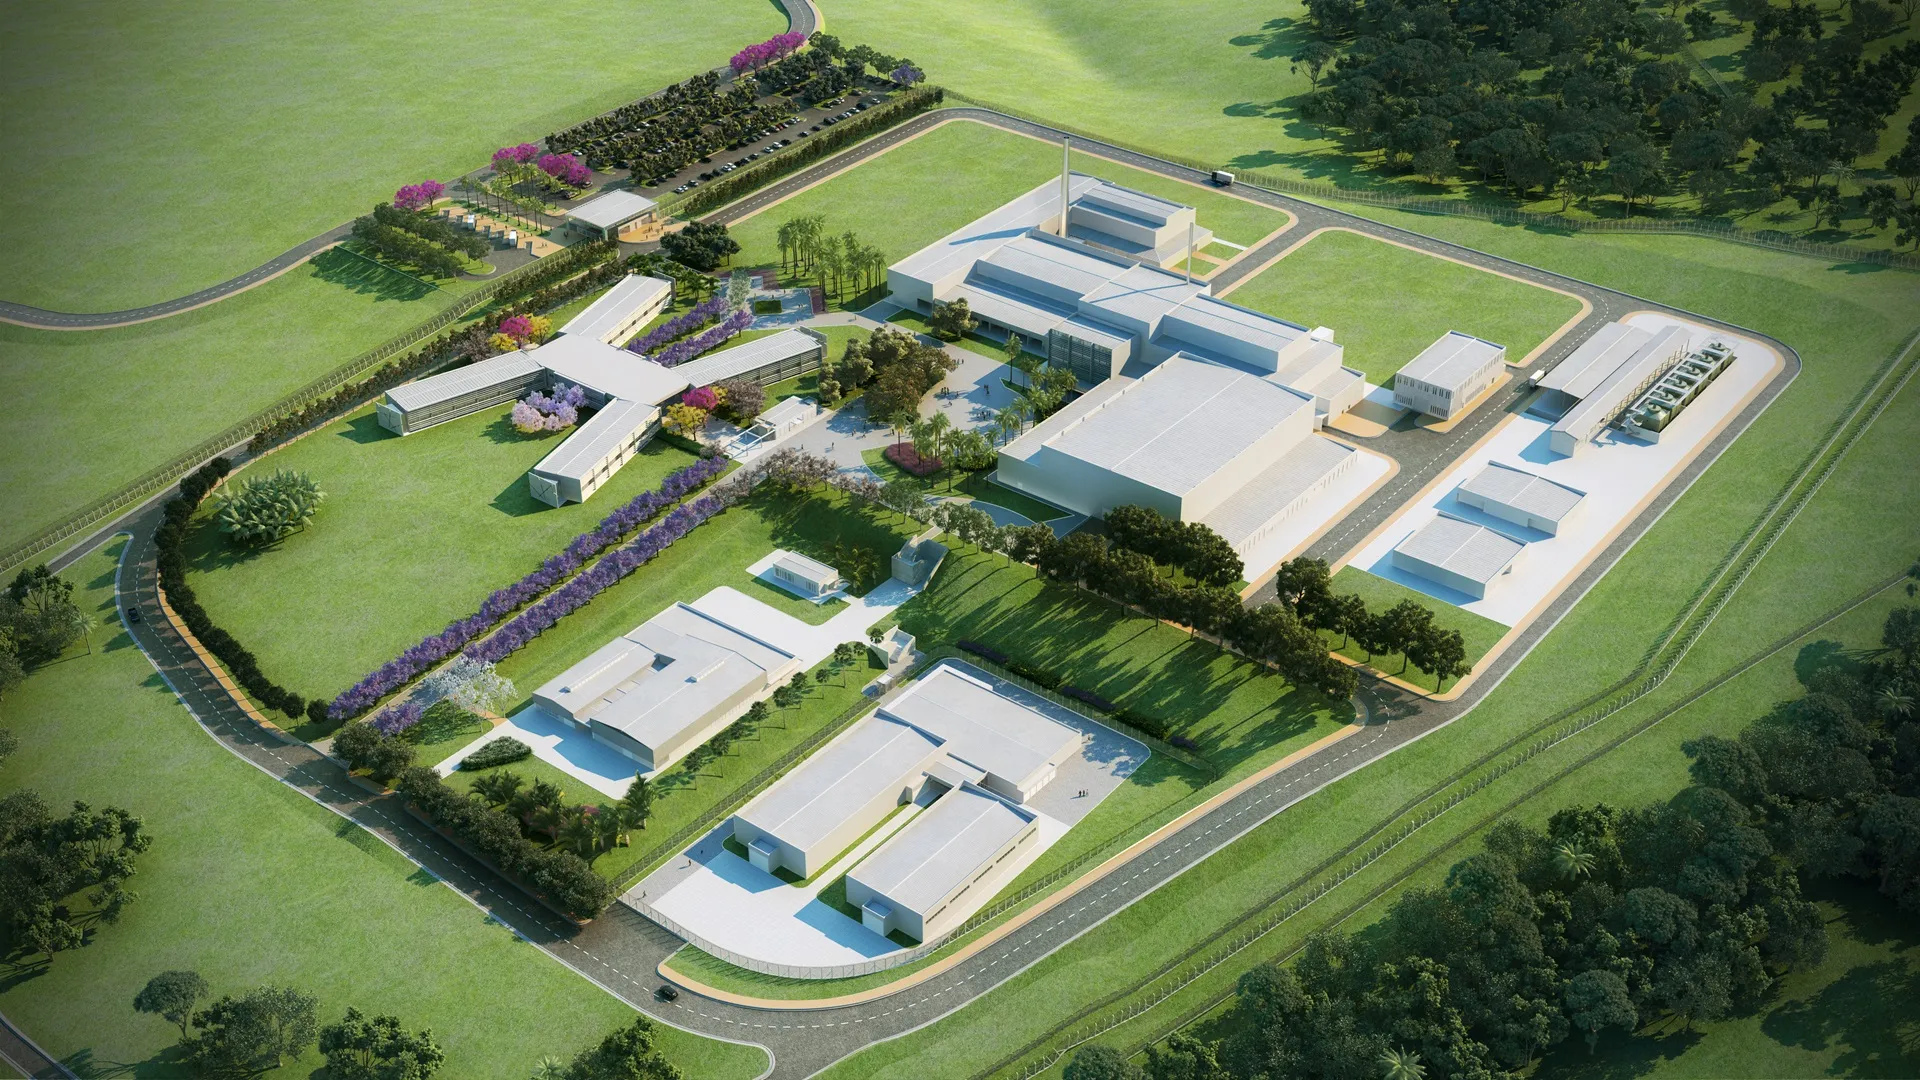
\includegraphics[width=\textwidth]{figures/rmb_vista_aerea.png}

\vspace{16pt}

% ---- Titulo grande, estilo capa de revista ----
\begin{center}
{\sffamily\bfseries\fontsize{24}{28}\selectfont\color{nurule}
REATOR MULTIPROP\'OSITO BRASILEIRO}\\[10pt]
{\sffamily\large RELAT\'ORIO PRELIMINAR DE AN\'ALISE DE SEGURAN\c{C}A}
\end{center}

\vfill
{\small\color{nugray}\itshape Vista a\'erea do complexo do RMB -- Ipero/SP (imagem ilustrativa do projeto).}\\[4pt]
\color{nurule}\rule{\textwidth}{0.6pt}
\restoregeometry
\clearpage

% =====================================================================
% capa.tex -- pagina de rosto / capa, inspirada na diagramacao de
% documentos do NRC (NUREG-1537) e do AP1000 DCD, sem reproduzir
% brasoes, selos ou logotipos oficiais.
% =====================================================================
\clearpage
\newgeometry{top=1.6cm,bottom=2.5cm,left=3.0cm,right=2.3cm}
\thispagestyle{empty}
\singlespacing
\begin{center}

\rule{\textwidth}{1.6pt}\\[2pt]
\rule{\textwidth}{0.6pt}\\[14pt]

{\sffamily\large COMISSÃO NACIONAL DE ENERGIA NUCLEAR}\\[2pt]
{\sffamily\small CNEN/RMB}

\vspace{0.8cm}

{\sffamily\bfseries\LARGE RELAT\'ORIO PRELIMINAR\\[3pt] DE AN\'ALISE DE SEGURAN\c{C}A}\\[8pt]
{\sffamily\normalsize (RPAS)}\\[3pt]
{\sffamily\normalsize Requerimento de Permiss\~ao de Constru\c{c}\~ao}

\vspace{0.6cm}

{\sffamily\bfseries\Large CAP\'ITULO 1}\\[4pt]
{\sffamily\large A INSTALA\c{C}\~AO}

\vspace{0.35cm}
{\sffamily\small PROPOSTA -- MINUTA DE TRABALHO PARA DISCUSS\~AO INTERNA}

\vspace{0.5cm}

\begin{tabular}{@{}>{\raggedright}p{0.32\textwidth}p{0.56\textwidth}@{}}
\textbf{Identifica\c{c}\~ao do documento:} & RMB-N00-00-LN-G-7240-RA-001 \\
\textbf{Revis\~ao:} & 0 (minuta) \\
\textbf{Data:} & Setembro de 2026 \\
\textbf{Idioma:} & Portugu\^es \\
\textbf{Refer\^encia de formato:} & USNRC NUREG-1537, Partes 1 e 2 \citep{nureg1537p1,nureg1537p2}\\
\end{tabular}

\vfill

\begin{minipage}{0.9\textwidth}
\centering\small
\textit{\textbf{AVISO: }Este documento \'e uma proposta preliminar de estrutura e conte\'udo para o
Cap\'itulo 1 do RPAS, elaborada pela FERMIUM TECNOLOGIA NUCLEAR com base no formato sugerido
pela NUREG-1537 (aplic\'avel a reatores n\~ao-de-pot\^encia / multi\-pro\-p\'osito) e na
apresenta\c{c}\~ao gr\'afica de Relat\'orios Finais de An\'alise de Seguran\c{c}a (FSAR) de
projetos certificados.}
\end{minipage}

\vspace{0.5cm}
\rule{\textwidth}{0.6pt}\\[2pt]
\rule{\textwidth}{1.6pt}

\end{center}
\restoregeometry
\clearpage


\pagestyle{plain}
\nusecbreaknopage{toc}{Sum\'ario}
\tableofcontents

\nusecbreak{lot}{Lista de Tabelas}
\listoftables

\nusecbreak{lof}{Lista de Figuras}
\listoffigures
\nuwritesectotal

\mainmatter
\gdef\nucursecid{}
% =====================================================================
% cap1.tex -- Capitulo 1: A Instalacao (The Facility)
% Estrutura de secoes 1.1 a 1.8 conforme NUREG-1537, Parte 1
% (Format and Content) \citep{nureg1537p1} e criterios de aceitacao
% da NUREG-1537, Parte 2 (Standard Review Plan) \citep{nureg1537p2}.
% =====================================================================
\chapter{A Instala\c{c}\~ao}
\nusecbreaknopage{1.1}{Se\c{c}\~ao 1.1}
\chapterbanner{1}{A Instala\c{c}\~ao}

Este cap\'itulo apresenta uma introdu\c{c}\~ao ao Relat\'orio Preliminar de
An\'alise de Seguran\c{c}a (RPAS) e \`a instala\c{c}\~ao, seguindo o formato
sugerido pela NUREG-1537, Parte~1, \emph{``Guidelines for Preparing and
Reviewing Applications for the Licensing of Non-Power Reactors: Format and
Content''} \citep{nureg1537p1}, e revisado em rela\c{c}\~ao aos crit\'erios de
aceita\c{c}\~ao da NUREG-1537, Parte~2, \emph{``Guidelines for Preparing and
Reviewing Applications for the Licensing of Non-Power Reactors: Standard
Review Plan and Acceptance Criteria''} \citep{nureg1537p2}. Este cap\'itulo \'e uma vis\~ao geral, ou resumo
executivo, dos temas tratados em detalhe nos cap\'itulos subsequentes do
RPAS; ele n\~ao substitui a discuss\~ao completa e as an\'alises
apresentadas naqueles cap\'itulos.
%\pagebreak

\begin{notaregulatoria}{Sobre esta proposta}
Este documento \'e um \textbf{modelo/proposta} (template) para o
Cap\'itulo~1 do RPAS, com trechos entre colchetes \texttt{[...]} a
serem preenchidos com os dados reais da instala\c{c}\~ao. A estrutura de
se\c{c}\~oes (\ref{sec:1.1} a \ref{sec:1.8}) segue integralmente a NUREG-1537, Parte~1
\citep{nureg1537p1}, que \'e voltada a reatores n\~ao-de-pot\^encia
(reatores de pesquisa e multiprop\'osito).
\end{notaregulatoria}

% =====================================================================
\section{Introdu\c{c}\~ao}
\label{sec:1.1}

[Nome do Requerente], uma [universidade / \'org\~ao governamental /
instituto de pesquisa / empresa], apresenta este Cap\'itulo~1 do
Relat\'orio Preliminar de An\'alise de Seguran\c{c}a (RPAS) em apoio a
uma solicita\c{c}\~ao de [permiss\~ao de constru\c{c}\~ao e licen\c{c}a de
opera\c{c}\~ao] para a [Nome da
Instala\c{c}\~ao/Reator], um [tipo de reator, p.ex., reator a \'agua
pressurizada sem boro sol\'uvel (SBF-PWR) / reator de pesquisa
multiprop\'osito tipo piscina aberta] com pot\^encia t\'ermica nominal de
[valor] MW(t) [e, se aplic\'avel, capacidade de pulso at\'e [valor]
MW(t) de pico], a ser instalado em [local/cidade, estado, pa\'is]. O uso
pretendido da instala\c{c}\~ao \'e [pesquisa, produ\c{c}\~ao de
rad\i s\'otopos, irradia\c{c}\~ao de materiais, pesquisa com feixes de
n\^eutrons, ensino e treinamento e/ou gera\c{c}\~ao de eletricidade,
conforme aplic\'avel].

As principais caracter\'isticas de seguran\c{c}a inerentes ou passivas do
projeto incluem [p.ex., coeficiente de temperatura do moderador
fortemente negativo, remo\c{c}\~ao do calor de decaimento por
circula\c{c}\~ao natural, sistemas passivos de resfriamento do n\'ucleo e
controle de reatividade sem boro sol\'uvel, apoiado em venenos
queim\'aveis e barras de controle]. Caracter\'isticas de projeto \'unicas
que distinguem esta instala\c{c}\~ao de reatores n\~ao-de-pot\^encia ou de
pot\^encia previamente licenciados incluem [listar, p.ex., elimina\c{c}\~ao
da fun\c{c}\~ao de bora\c{c}\~ao do sistema de controle qu\'imico e de
volume, n\'ucleo compacto com retroalimenta\c{c}\~ao de reatividade
negativa refor\c{c}ada, ou miss\~ao combinada de pesquisa/irradia\c{c}\~ao].
Esses temas s\~ao tratados integralmente nos Cap\'itulos~2 a~17 deste
RPAS, aos quais esta se\c{c}\~ao remete ao longo do texto.

\subsection*{Enquadramento regulat\'orio do RMB}
\label{sec:1.1.enquadramento}

Antes de entrar no detalhamento dos itens ~\ref{sec:1.1} a ~\ref{sec:1.8}, cabe situar onde o
RMB se encaixa nas categorias que a NUREG-1537 \citep{nureg1537p1,nureg1537p2} e o \emph{Interim Staff
Guidance Augmenting NUREG-1537}
\citep[NPR-ISG-2011-002;][]{isgnureg1537p1,isgnureg1537p2} -- aqui referido, por
brevidade, como \textbf{ISG-NUREG-1537} -- que a complementa efetivamente
reconhecem -- porque nenhuma das duas normas usa a express\~ao ``reator
multiprop\'osito'' como categoria regulat\'oria pr\'opria.

A NUREG-1537 trabalha com uma divis\~ao bin\'aria dentro do guarda-chuva
de reator n\~ao-de-pot\^encia: de um lado o reator de pesquisa
(\emph{research reactor}), de outro a instala\c{c}\~ao de teste
(\emph{testing facility}), esta \'ultima sujeita a exig\^encias
adicionais -- declara\c{c}\~ao de impacto ambiental, audi\^encia de
licenciamento e revis\~ao pelo \emph{Advisory Committee on Reactor
Safeguards} (ACRS). O crit\'erio que separa as duas categorias \'e
objetivo, n\~ao nominal: o 10~CFR~50.2 -- \citep{cfr10p50} -- enquadra como \emph{testing
facility} qualquer reator com pot\^encia t\'ermica acima de 1~MW(t) e com
instala\c{c}\~ao experimental \emph{in-core} de se\c{c}\~ao transversal
superior a 16~polegadas quadradas. Com pot\^encia de projeto de 30~MW(t)
e m\'ultiplos canais de irradia\c{c}\~ao \emph{in-core} e
\emph{in-reflector}, o RMB tende a se enquadrar nessa categoria mais
rigorosa -- n\~ao por ser ``multiprop\'osito'', mas por pot\^encia e por
ter instala\c{c}\~oes experimentais internas ao n\'ucleo acima do limiar
do regulamento.
%esse enquadramento deve ser confirmado formalmente com o
%\'org\~ao regulador nacional antes %da submiss\~ao deste RPAS.

O ISG-NUREG-1537 acrescenta uma segunda camada a
essa classifica\c{c}\~ao. Ele foi escrito para cobrir, entre outros
cen\'arios, exatamente o do RMB: um reator \textbf{heterog\^eneo}
(n\'ucleo com elementos combust\'iveis tipo placa, n\~ao solu\c{c}\~ao
homog\^enea) que irradia alvos de ur\^anio pouco enriquecido (LEU) para
produ\c{c}\~ao de molibd\^enio-99, com o material irradiado
posteriormente processado em uma instala\c{c}\~ao de separa\c{c}\~ao
radioqu\'imica associada. Para esse cen\'ario -- que o pr\'oprio ISG-NUREG-1537
descreve como produ\c{c}\~ao de Mo-99 por fiss\~ao de material nuclear
especial em alvos LEU irradiados em reatores n\~ao-de-pot\^encia
existentes ou novos --, o tratamento \'e expl\'icito: o reator em si
continua coberto pelo escopo padr\~ao da NUREG-1537, com orienta\c{c}\~ao
adicional m\'inima; j\'a a instala\c{c}\~ao onde ocorre a separa\c{c}\~ao
do radiois\'otopo passa a ser tratada, para fins de licenciamento, como
uma instala\c{c}\~ao de produ\c{c}\~ao (\emph{production facility}) sob o
10~CFR Parte~50 (\citealp{cfr10p50}), sujeita aos cap\'itulos e crit\'erios de aceita\c{c}\~ao
que o ISG-NUREG-1537 acrescenta especificamente para esse tipo de instala\c{c}\~ao.

Na pr\'atica, isso separa o RMB em dois objetos de licenciamento com
tratamento regulat\'orio distinto, ainda que fisicamente cont\'iguos: o
pr\'edio do reator, onde a NUREG-1537 domina quase sem altera\c{c}\~ao
(com os complementos ``a1'' do ISG-NUREG-1537 para reator heterog\^eneo, quando
aplic\'aveis aos Cap\'itulos~4, 5, 6, 8 e~9), e a instala\c{c}\~ao de
produ\c{c}\~ao de radiois\'otopos, onde o ISG-NUREG-1537 \'e a refer\^encia
prim\'aria. Essa distin\c{c}\~ao \'e consistente com a estrat\'egia de
licenciamento faseado j\'a registrada no anexo deste cap\'itulo (ver
``Anexo -- Estrat\'egia de Licenciamento Faseado''): o escopo inicial
deste RPAS, limitado ao pr\'edio do reator, corresponde ao objeto onde a
NUREG-1537 base j\'a basta; a instala\c{c}\~ao de produ\c{c}\~ao de Mo-99,
quando entrar em escopo, dever\'a ser tratada com o apoio direto do
ISG-NUREG-1537, mapeado no \apref{apA}{A} deste cap\'itulo.

\begin{tabelaaceitacao}{\ref{sec:1.1}}{Introdu\c{c}\~ao}
1 & O prop\'osito do RPAS deve estar claramente declarado. \\
2 & O requerente deve estar identificado (nome, natureza jur\'idica). \\
3 & A localiza\c{c}\~ao, o prop\'osito e o uso da instala\c{c}\~ao devem
     estar brevemente descritos. \\
4 & As caracter\'isticas b\'asicas da instala\c{c}\~ao que afetam as
     considera\c{c}\~oes de licenciamento devem estar brevemente
     discutidas. \\
5 & As caracter\'isticas de projeto ou de localiza\c{c}\~ao voltadas a
     endere\c{c}ar preocupa\c{c}\~oes b\'asicas de seguran\c{c}a devem
     estar delineadas. \\
6 & Caracter\'isticas de seguran\c{c}a \'unicas do projeto, diferentes de
     instala\c{c}\~oes n\~ao-de-pot\^encia previamente licenciadas, devem
     estar destacadas. \\
\end{tabelaaceitacao}

\begin{tabelaresumo}{\ref{sec:1.1}}{Introdu\c{c}\~ao}
Identifica\c{c}\~ao do requerente & Nome, natureza jur\'idica (universidade,
  \'org\~ao governamental, instituto, empresa) e, quando aplic\'avel, o
  arranjo de propriedade/opera\c{c}\~ao da instala\c{c}\~ao. \\
Prop\'osito e uso pretendido & Miss\~ao declarada do reator (pesquisa,
  irradia\c{c}\~ao, produ\c{c}\~ao de is\'otopos, ensino, gera\c{c}\~ao de
  pot\^encia). \\
Localiza\c{c}\~ao geogr\'afica & Local, munic\'ipio/estado/pa\'is do
  s\'itio proposto. \\
Tipo e pot\^encia do reator & Tecnologia (p.ex. PWR sem boro sol\'uvel,
  piscina aberta), pot\^encia t\'ermica nominal e, se aplic\'avel,
  capacidade de pulso. \\
Caracter\'isticas de seguran\c{c}a inerentes/passivas & Elementos de
  seguran\c{c}a intr\'insecos ao projeto que reduzem a depend\^encia de
  a\c{c}\~ao ativa ou humana. \\
Caracter\'isticas \'unicas de projeto & Aspectos que diferenciam esta
  instala\c{c}\~ao de projetos j\'a licenciados e que merecer\~ao aten\c{c}\~ao
  espec\'ifica do revisor. \\
\end{tabelaresumo}

\begin{tabelaapendices}{\ref{sec:1.1}}{Introdu\c{c}\~ao}
Cap\'itulos 2--17 do RPAS & Confirmar que cada tema mencionado nesta
  se\c{c}\~ao (local, tipo de reator, pot\^encia, seguran\c{c}a passiva)
  \'e de fato detalhado e \'e consistente com o cap\'itulo correspondente. &
  Pendente \\
NUREG-1537, Parte~1, \S1.1 \citep{nureg1537p1} & Verificar aderência ao
  conte\'udo m\'inimo exigido para a introdu\c{c}\~ao. & Pendente \\
NUREG-1537, Parte~2, \S1.1 \citep{nureg1537p2} & Verificar os crit\'erios
  de aceita\c{c}\~ao aplic\'aveis antes da submiss\~ao. & Pendente \\
\end{tabelaapendices}

\begin{avaliacaointerim}
O ISG-NUREG-1537 amplia o escopo desta se\c{c}\~ao:
onde a NUREG-1537 fala em caracter\'isticas de seguran\c{c}a inerentes ou
passivas do reator, o ISG-NUREG-1537 passa a exigir que as caracter\'isticas
inerentes/passivas da instala\c{c}\~ao de produ\c{c}\~ao de radiois\'otopos
associada tamb\'em sejam descritas aqui, quando aplic\'avel ao escopo do
RPAS. N\~ao h\'a altera\c{c}\~ao na estrutura da se\c{c}\~ao nem novo
crit\'erio de aceita\c{c}\~ao formal -- apenas amplia\c{c}\~ao do escopo
textual, j\'a refletida no \apref{apA}{A}. Como o escopo inicial deste RPAS
est\'a limitado ao pr\'edio do reator (ver Anexo -- Estrat\'egia de
Licenciamento Faseado), essa amplia\c{c}\~ao passa a valer integralmente
apenas quando a instala\c{c}\~ao de produ\c{c}\~ao de Mo-99 for
incorporada em fase posterior.
\end{avaliacaointerim}

% =====================================================================
\nusecbreak{1.2}{Se\c{c}\~ao 1.2}
\section{Resumo e Conclus\~oes sobre as Principais Considera\c{c}\~oes de
Seguran\c{c}a}
\label{sec:1.2}

Esta se\c{c}\~ao apresenta os crit\'erios de seguran\c{c}a, as principais
considera\c{c}\~oes de seguran\c{c}a e as conclus\~oes decorrentes para a
instala\c{c}\~ao, incluindo discuss\~oes breves sobre: as consequ\^encias
da opera\c{c}\~ao e uso do reator e os m\'etodos empregados para garantir
a seguran\c{c}a; as considera\c{c}\~oes de seguran\c{c}a que influenciaram
a escolha do s\'itio, do tipo de reator e combust\'ivel, da pot\^encia
t\'ermica e do tipo de edifica\c{c}\~ao; as caracter\'isticas de
seguran\c{c}a inerentes ou passivas projetadas para proteger a sa\'ude e
seguran\c{c}a do p\'ublico, da equipe e do meio ambiente; as bases de
projeto de sistemas e componentes que promovem a opera\c{c}\~ao e o
desligamento seguros; e os acidentes potenciais na instala\c{c}\~ao,
incluindo o acidente hipot\'etico m\'aximo (MHA) [e, quando aplic\'avel,
outros eventos-base de projeto limitantes], bem como as caracter\'isticas
de projeto que os previnem ou mitigam.

N\~ao se espera que nenhuma exposi\c{c}\~ao decorrente da opera\c{c}\~ao
normal exceda os limites do [10~CFR Parte~20 \citep{cfr10p20} / regulamento
nacional de radioprote\c{c}\~ao aplic\'avel], e a instala\c{c}\~ao \'e
projetada e ser\'a operada de acordo com o princ\'ipio ALARA (t\~ao baixo
quanto razoavelmente exequ\'ivel). Essas discuss\~oes constituem uma
vis\~ao geral; as an\'alises detalhadas encontram-se nos
Cap\'itulos~3 a~13 deste RPAS.
\begin{tabelaaceitacao}{\ref{sec:1.2}}{Resumo das considera\c{c}\~oes de seguran\c{c}a}
1 & Caracter\'isticas de projeto suficientes devem estar inclu\'idas para
     proteger a sa\'ude e a seguran\c{c}a do p\'ublico. \\
2 & Nenhuma exposi\c{c}\~ao decorrente de opera\c{c}\~ao normal deve
     exceder os limites regulat\'orios aplic\'aveis, observado o
     princ\'ipio ALARA. \\
3 & Os acidentes potenciais devem estar brevemente discutidos. \\
4 & Todos os modos de opera\c{c}\~ao e eventos capazes de causar liberações
     radiol\'ogicas significativas e exposi\c{c}\~ao do p\'ublico devem
     estar discutidos. \\
\end{tabelaaceitacao}

\begin{tabelaresumo}{\ref{sec:1.2}}{Resumo das considera\c{c}\~oes de seguran\c{c}a}
Crit\'erios de seguran\c{c}a declarados & Base regulat\'oria e princ\'ipios
  de projeto adotados (defesa em profundidade, ALARA, margens de
  seguran\c{c}a). \\
Considera\c{c}\~oes que influenciaram o projeto & Justificativas de
  escolha do s\'itio, tipo de reator/combust\'ivel, pot\^encia e
  edifica\c{c}\~ao. \\
Caracter\'isticas inerentes/passivas & Mecanismos que independem de a\c{c}\~ao
  ativa (retroalimenta\c{c}\~ao de reatividade, remo\c{c}\~ao passiva de
  calor). \\
Acidente hipot\'etico m\'aximo (MHA) & Cen\'ario acidental mais restritivo
  considerado no dimensionamento das barreiras de seguran\c{c}a. \\
Conclus\~ao de conformidade & Declara\c{c}\~ao de que as doses previstas
  respeitam os limites regulat\'orios em todas as condi\c{c}\~oes
  avaliadas. \\
\end{tabelaresumo}

\begin{tabelaapendices}{\ref{sec:1.2}}{Resumo das considera\c{c}\~oes de seguran\c{c}a}
Cap\'itulo 13 -- An\'alise de Acidentes & Confirmar que o acidente
  hipot\'etico m\'aximo (MHA) citado aqui corresponde \`a an\'alise
  detalhada do Cap\'itulo 13. & Pendente \\
Cap\'itulo 6 -- Caracter\'isticas de Seguran\c{c}a Projetadas & Verificar
  consist\^encia entre as caracter\'isticas passivas resumidas aqui e a
  descri\c{c}\~ao detalhada. & Pendente \\
10~CFR Parte~20 (ou equivalente nacional) \citep{cfr10p20} & Confirmar que
  os limites de dose citados est\~ao corretos e atualizados. & Pendente \\
\end{tabelaapendices}

\begin{avaliacaointerim}
Esta \'e a se\c{c}\~ao em que o ISG-NUREG-1537 introduz a mudan\c{c}a mais
substantiva para o Cap\'itulo~1: al\'em de reformular itens de texto
corrido da NUREG-1537 para incluir explicitamente a instala\c{c}\~ao de
produ\c{c}\~ao de radiois\'otopos, o ISG-NUREG-1537 acrescenta, na Parte~2
(crit\'erios de aceita\c{c}\~ao), uma \'area de revis\~ao inteiramente
nova -- a vis\~ao geral de processo (\emph{process overview}) da
instala\c{c}\~ao de produ\c{c}\~ao, cobrindo a rela\c{c}\~ao entre os
principais processos qu\'imicos/mec\^anicos e o material licenci\'avel
envolvido, a localiza\c{c}\~ao das edifica\c{c}\~oes dos principais
componentes de processo (apoiada em desenhos), e a marca\c{c}\~ao de
eventuais informa\c{c}\~oes propriet\'arias ou sens\'iveis. Diferentemente
das demais se\c{c}\~oes, este n\~ao \'e apenas um ajuste de terminologia:
se e quando a instala\c{c}\~ao de produ\c{c}\~ao de Mo-99 entrar no
escopo deste RPAS, esta se\c{c}\~ao vai exigir um par\'agrafo pr\'oprio de
vis\~ao geral de processo, com n\'ivel de detalhe consistente com o
resumo da an\'alise de seguran\c{c}a integrada (ISA) e com o
Cap\'itulo~13. Essa necessidade j\'a est\'a sinalizada no \apref{apA}{A}.
\end{avaliacaointerim}

% =====================================================================
\nusecbreak{1.3}{Se\c{c}\~ao 1.3}
\section{Descri\c{c}\~ao Geral}
\label{sec:1.3}

Esta se\c{c}\~ao descreve brevemente a instala\c{c}\~ao do reator,
incluindo: (1) a localiza\c{c}\~ao geogr\'afica; (2) as principais
caracter\'isticas do s\'itio; (3) os principais crit\'erios de projeto,
caracter\'isticas operacionais e sistemas de seguran\c{c}a; (4) quaisquer
caracter\'isticas de seguran\c{c}a projetadas (\textit{engineered safety
features}); (5) sistemas de instrumenta\c{c}\~ao, controle e el\'etricos;
(6) o sistema de refrigera\c{c}\~ao do reator e demais sistemas
auxiliares; (7) as provis\~oes de gerenciamento de rejeitos radioativos e
prote\c{c}\~ao radiol\'ogica; e (8) as instala\c{c}\~oes e capacidades
experimentais [ou, no caso de um projeto de reator de pot\^encia, os
sistemas do \textit{balance-of-plant}]. O arranjo geral das principais
estruturas e equipamentos \'e indicado por meio de plantas e cortes nas
Figuras~1-[n] a~1-[n]. As caracter\'isticas de seguran\c{c}a de maior
interesse -- tais como [caracter\'isticas incomuns do s\'itio, o projeto
de cont\^enc\~ao/confinamento, aspectos in\'editos do projeto do reator ou
instala\c{c}\~oes experimentais \'unicas] -- s\~ao brevemente destacadas a
seguir; a discuss\~ao e a an\'alise completas encontram-se nos
cap\'itulos subsequentes deste RPAS, aos quais esta se\c{c}\~ao remete.
\begin{tabelaaceitacao}{\ref{sec:1.3}}{Descri\c{c}\~ao geral da instala\c{c}\~ao}
1 & Devem estar brevemente descritos: localiza\c{c}\~ao geogr\'afica,
     caracter\'isticas do s\'itio, crit\'erios de projeto, sistemas de
     seguran\c{c}a, instrumenta\c{c}\~ao/controle/el\'etrica, sistemas de
     refrigera\c{c}\~ao e auxiliares, gerenciamento de rejeitos e
     prote\c{c}\~ao radiol\'ogica, e instala\c{c}\~oes experimentais. \\
2 & O arranjo geral das principais estruturas e equipamentos deve estar
     indicado por plantas e cortes (desenhos de eleva\c{c}\~ao). \\
3 & As caracter\'isticas de seguran\c{c}a de maior interesse devem estar
     brevemente identificadas. \\
4 & Caracter\'isticas incomuns do s\'itio, da cont\^enc\~ao, do projeto do
     reator ou de instala\c{c}\~oes experimentais \'unicas devem estar
     destacadas. \\
\end{tabelaaceitacao}

\begin{tabelaresumo}{\ref{sec:1.3}}{Descri\c{c}\~ao geral da instala\c{c}\~ao}
S\'itio & Localiza\c{c}\~ao e principais caracter\'isticas f\'isicas,
  demogr\'aficas e ambientais (detalhado no Cap\'itulo 2). \\
Sistemas de seguran\c{c}a e projeto & Vis\~ao geral dos crit\'erios de
  projeto e sistemas de seguran\c{c}a (detalhado nos Cap\'itulos 3, 4 e 6). \\
Instrumenta\c{c}\~ao, controle e el\'etrica & Vis\~ao geral (detalhado nos
  Cap\'itulos 7 e 8). \\
Refrigera\c{c}\~ao e auxiliares & Sistemas de remo\c{c}\~ao de calor e
  suporte (detalhado nos Cap\'itulos 5 e 9). \\
Rejeitos e radioprote\c{c}\~ao & Provis\~oes de gerenciamento e prote\c{c}\~ao
  radiol\'ogica (detalhado no Cap\'itulo 11). \\
Instala\c{c}\~oes experimentais & Capacidades experimentais/irradia\c{c}\~ao
  (detalhado no Cap\'itulo 10), quando aplic\'avel. \\
Desenhos de arranjo geral & Plantas e cortes indicando a disposi\c{c}\~ao
  das principais estruturas e equipamentos. \\
\end{tabelaresumo}

\begin{tabelaapendices}{\ref{sec:1.3}}{Descri\c{c}\~ao geral da instala\c{c}\~ao}
Cap\'itulos 2 a 11 do RPAS & Confirmar consist\^encia entre o resumo desta
  se\c{c}\~ao e o conte\'udo detalhado de cada cap\'itulo referenciado. &
  Pendente \\
Figuras 1-[n] a 1-[n] (plantas e cortes) & Verificar exist\^encia,
  numera\c{c}\~ao e atualiza\c{c}\~ao dos desenhos de arranjo geral. &
  Pendente \\
\end{tabelaapendices}

\begin{avaliacaointerim}
O ISG-NUREG-1537 segue o mesmo padr\~ao de amplia\c{c}\~ao j\'a visto na
Se\c{c}\~ao~\ref{sec:1.1}: a descri\c{c}\~ao geral da instala\c{c}\~ao, tal como
exigida pela NUREG-1537, deve ser expandida para tamb\'em cobrir a
instala\c{c}\~ao de produ\c{c}\~ao de radiois\'otopos, quando esta
estiver no escopo do RPAS. N\~ao h\'a crit\'erio de aceita\c{c}\~ao
adicional espec\'ifico para esta se\c{c}\~ao na Parte~2 do ISG-NUREG-1537, nem
altera\c{c}\~ao estrutural -- apenas a mesma substitui\c{c}\~ao de leitura
(``reator'' passa a significar ``reator e/ou instala\c{c}\~ao de
produ\c{c}\~ao de radiois\'otopos'') j\'a registrada na Se\c{c}\~ao~\ref{sec:1.1}.
\end{avaliacaointerim}

% =====================================================================
\nusecbreak{1.4}{Se\c{c}\~ao 1.4}
\section{Instala\c{c}\~oes e Equipamentos Compartilhados}
\label{sec:1.4}

Esta se\c{c}\~ao descreve brevemente: sistemas e equipamentos
compartilhados com instala\c{c}\~oes n\~ao abrangidas por este RPAS ou
pela licen\c{c}a/certifica\c{c}\~ao (p.ex., sistemas de purifica\c{c}\~ao
de \'agua; suprimento el\'etrico; sistemas de aquecimento, ventila\c{c}\~ao
e ar-condicionado; e o edif\'icio que abriga a sala do reator); qualquer
outro reator, conjunto subcr\'itico, instala\c{c}\~ao de irradia\c{c}\~ao
ou c\'elula quente localizados dentro da estrutura de
confinamento/cont\^enc\~ao ou da \'area restrita a que este RPAS se
aplica; e quaisquer barreiras de seguran\c{c}a ou provis\~oes especiais de
isolamento para as instala\c{c}\~oes e equipamentos compartilhados. [Caso
n\~ao haja instala\c{c}\~oes ou equipamentos compartilhados, isso deve ser
declarado explicitamente.] As descri\c{c}\~oes completas e quaisquer
implica\c{c}\~oes de seguran\c{c}a decorrentes do compartilhamento s\~ao
avaliadas nos cap\'itulos pertinentes deste RPAS, aos quais esta se\c{c}\~ao
remete.
\begin{tabelaaceitacao}{\ref{sec:1.4}}{Instala\c{c}\~oes e equipamentos compartilhados}
1 & A instala\c{c}\~ao deve ser projetada para acomodar todos os usos ou
     falhas das instala\c{c}\~oes compartilhadas sem degrada\c{c}\~ao das
     caracter\'isticas de seguran\c{c}a do reator. \\
2 & O projeto deve evitar condi\c{c}\~oes em que a contamina\c{c}\~ao
     possa se propagar para as instala\c{c}\~oes ou equipamentos
     compartilhados. \\
3 & Onde necess\'ario, as barreiras devem estar brevemente descritas para
     garantir o atendimento aos dois crit\'erios anteriores. \\
\end{tabelaaceitacao}

\begin{tabelaresumo}{\ref{sec:1.4}}{Instala\c{c}\~oes e equipamentos compartilhados}
Sistemas compartilhados & Lista de sistemas/equipamentos compartilhados
  (\'agua, energia el\'etrica, HVAC, edifica\c{c}\~ao) e seus outros
  usu\'arios. \\
Instala\c{c}\~oes co-localizadas & Outros reatores, conjuntos subcr\'iticos
  ou instala\c{c}\~oes de irradia\c{c}\~ao no mesmo pr\'edio/\'area
  restrita. \\
Barreiras e isolamento & Provis\~oes que impedem a propaga\c{c}\~ao de
  contamina\c{c}\~ao ou a perda de fun\c{c}\~ao de seguran\c{c}a por conta
  do compartilhamento. \\
\end{tabelaresumo}

\begin{tabelaapendices}{\ref{sec:1.4}}{Instala\c{c}\~oes e equipamentos compartilhados}
Cap\'itulo 9 -- Sistemas Auxiliares & Confirmar descri\c{c}\~ao detalhada
  dos sistemas compartilhados citados aqui. & Pendente \\
Cap\'itulo 13 -- An\'alise de Acidentes & Verificar se falhas de sistemas
  compartilhados foram avaliadas quanto \`a libera\c{c}\~ao de material
  radioativo. & Pendente \\
\end{tabelaapendices}

\begin{avaliacaointerim}
O ISG-NUREG-1537 trata as Se\c{c}\~oes~\ref{sec:1.4} a~\ref{sec:1.8} em bloco, sem acr\'escimo
espec\'ifico a esta se\c{c}\~ao al\'em da mesma amplia\c{c}\~ao
terminol\'ogica j\'a aplicada \`as se\c{c}\~oes anteriores: onde a
NUREG-1537 menciona ``reator'', o ISG-NUREG-1537 entende que a men\c{c}\~ao
cobre tamb\'em a instala\c{c}\~ao de produ\c{c}\~ao de radiois\'otopos,
quando aplic\'avel. Para esta se\c{c}\~ao em particular, isso significa
que sistemas e equipamentos eventualmente compartilhados entre o pr\'edio
do reator e uma futura instala\c{c}\~ao de produ\c{c}\~ao de Mo-99 devem,
quando essa instala\c{c}\~ao entrar em escopo, ser descritos aqui nos
mesmos termos j\'a usados para outras instala\c{c}\~oes compartilhadas.
N\~ao h\'a mudan\c{c}a estrutural decorrente do ISG-NUREG-1537 nesta se\c{c}\~ao.
\end{avaliacaointerim}

% =====================================================================
\nusecbreak{1.5}{Se\c{c}\~ao 1.5}
\section{Compara\c{c}\~ao com Instala\c{c}\~oes Similares}
\label{sec:1.5}

Esta se\c{c}\~ao descreve brevemente as principais semelhan\c{c}as entre
esta instala\c{c}\~ao e outras instala\c{c}\~oes, particularmente aquelas
licenciadas pela [autoridade regulat\'oria nacional] ou projetadas e
operadas por organiza\c{c}\~oes de pesquisa reconhecidas. S\~ao
comparados os principais par\^ametros de projeto, os sistemas de
seguran\c{c}a do reator, as caracter\'isticas de seguran\c{c}a projetadas
e os sistemas de instrumenta\c{c}\~ao e controle. O hist\'orico
operacional das instala\c{c}\~oes de refer\^encia \'e brevemente citado
para demonstrar a seguran\c{c}a e a confiabilidade da abordagem de
projeto adotada. Caracter\'isticas de projeto, experi\^encia operacional
e testes e experimentos das instala\c{c}\~oes de refer\^encia [p.ex.,
listar instala\c{c}\~oes/tecnologias de refer\^encia] s\~ao utilizados
para embasar as an\'alises apresentadas nos cap\'itulos aplic\'aveis
deste RPAS.
\begin{tabelaaceitacao}{\ref{sec:1.5}}{Compara\c{c}\~ao com instala\c{c}\~oes similares}
1 & As compara\c{c}\~oes devem demonstrar que a instala\c{c}\~ao proposta
     n\~ao excede o envelope de seguran\c{c}a das instala\c{c}\~oes
     similares. \\
2 & Deve haver garantia razo\'avel de que as exposi\c{c}\~oes
     radiol\'ogicas do p\'ublico n\~ao excedem os regulamentos e as
     diretrizes ALARA da instala\c{c}\~ao proposta. \\
\end{tabelaaceitacao}

\begin{tabelaresumo}{\ref{sec:1.5}}{Compara\c{c}\~ao com instala\c{c}\~oes similares}
Instala\c{c}\~oes de refer\^encia & Lista das instala\c{c}\~oes similares
  utilizadas como base comparativa (tipo, pot\^encia, tecnologia,
  status de licenciamento). \\
Par\^ametros comparados & Par\^ametros de projeto, sistemas de seguran\c{c}a,
  instrumenta\c{c}\~ao/controle e desempenho de combust\'ivel. \\
Hist\'orico operacional & Evid\^encias de opera\c{c}\~ao segura e
  confi\'avel nas instala\c{c}\~oes de refer\^encia. \\
Conclus\~ao comparativa & Declara\c{c}\~ao de que o projeto proposto n\~ao
  excede o envelope de seguran\c{c}a j\'a validado. \\
\end{tabelaresumo}

\begin{tabelaapendices}{\ref{sec:1.5}}{Compara\c{c}\~ao com instala\c{c}\~oes similares}
Cap\'itulo 4 -- Descri\c{c}\~ao do Reator & Confirmar base de aceita\c{c}\~ao
  do desempenho do combust\'ivel por compara\c{c}\~ao. & Pendente \\
Cap\'itulo 6 -- Caracter\'isticas de Seguran\c{c}a Projetadas & Confirmar
  base de compara\c{c}\~ao dos sistemas de mitiga\c{c}\~ao de acidentes. &
  Pendente \\
Cap\'itulo 7 -- Instrumenta\c{c}\~ao e Controle & Confirmar base de
  compara\c{c}\~ao de redund\^ancia/diversidade de instrumenta\c{c}\~ao. &
  Pendente \\
\end{tabelaapendices}

\begin{avaliacaointerim}
Diferentemente da amplia\c{c}\~ao gen\'erica aplicada \`as demais
se\c{c}\~oes do bloco \ref{sec:1.4}--\ref{sec:1.8}, a Se\c{c}\~ao~\ref{sec:1.5} recebe do ISG-NUREG-1537 uma
orienta\c{c}\~ao espec\'ifica: a lista de instala\c{c}\~oes de
refer\^encia para compara\c{c}\~ao, hoje limitada a reatores heterog\^eneos
n\~ao-de-pot\^encia, deve incluir tamb\'em instala\c{c}\~oes ou
opera\c{c}\~oes de produ\c{c}\~ao de radiois\'otopos compar\'aveis, quando
aplic\'avel. O ISG-NUREG-1537 lista ainda comparadores espec\'ificos para
reatores homog\^eneos aquosos (AHR) -- LOPO, HYPO, SUPO, TRACY e HRE --
mas esses n\~ao se aplicam ao RMB, que \'e um reator heterog\^eneo tipo
piscina, n\~ao um AHR; a distin\c{c}\~ao fica registrada aqui para evitar
compara\c{c}\~ao indevida. A mudan\c{c}a pr\'atica, quando a
instala\c{c}\~ao de produ\c{c}\~ao de Mo-99 entrar em escopo, \'e incluir
na tabela-resumo desta se\c{c}\~ao ao menos uma refer\^encia de
instala\c{c}\~ao de produ\c{c}\~ao de radiois\'otopos compar\'avel (por
exemplo, produtores de Mo-99 baseados em alvos LEU j\'a licenciados
internacionalmente).
\end{avaliacaointerim}

% =====================================================================
\nusecbreak{1.6}{Se\c{c}\~ao 1.6}
\section{Resumo das Opera\c{c}\~oes}
\label{sec:1.6}

Esta se\c{c}\~ao discute brevemente as opera\c{c}\~oes planejadas do
reator, os programas experimentais e a miss\~ao da instala\c{c}\~ao. As
opera\c{c}\~oes propostas s\~ao importantes para estimar par\^ametros como
tempo total de opera\c{c}\~ao, n\'ivel de pot\^encia, modo de opera\c{c}\~ao
(cont\'inuo, sob demanda ou pulsado) e a quantidade e o tipo de materiais
radioativos subprodutos gerados. [Caso a solicita\c{c}\~ao seja de
renova\c{c}\~ao de licen\c{c}a, esta se\c{c}\~ao deve refletir os planos
operacionais atuais e propostos.] Caso considera\c{c}\~oes de seguran\c{c}a
analisadas em cap\'itulos posteriores deste RPAS limitem o cronograma de
opera\c{c}\~ao do reator, esse fato \'e registrado aqui e referenciado ao
cap\'itulo aplic\'avel e \`as especifica\c{c}\~oes t\'ecnicas
(Cap\'itulo~14).
\begin{tabelaaceitacao}{\ref{sec:1.6}}{Resumo das opera\c{c}\~oes}
1 & O requerente deve demonstrar a consist\^encia das opera\c{c}\~oes
     propostas com as premissas adotadas nos cap\'itulos posteriores do
     RPAS, incluindo os efeitos sobre a integridade do reator e as
     exposi\c{c}\~oes radiol\'ogicas potenciais. \\
2 & O requerente deve demonstrar que a opera\c{c}\~ao proposta do reator
     foi considerada de forma conservadora no projeto e nas an\'alises de
     seguran\c{c}a. \\
3 & (Renova\c{c}\~ao) As opera\c{c}\~oes propostas devem ser consistentes
     com as premissas dos cap\'itulos posteriores do RPAS. \\
\end{tabelaaceitacao}

\begin{tabelaresumo}{\ref{sec:1.6}}{Resumo das opera\c{c}\~oes}
Miss\~ao e programas & Finalidade operacional (pesquisa, irradia\c{c}\~ao,
  produ\c{c}\~ao de is\'otopos, gera\c{c}\~ao) e programas experimentais
  previstos. \\
Regime de opera\c{c}\~ao & Cont\'inuo, sob demanda ou pulsado; fator de
  capacidade estimado. \\
Invent\'ario de produtos de fiss\~ao & Base assumida para o calor de
  decaimento e para os efluentes radioativos liberados. \\
Limita\c{c}\~oes de opera\c{c}\~ao & Restri\c{c}\~oes impostas por
  considera\c{c}\~oes de seguran\c{c}a e sua base nas especifica\c{c}\~oes
  t\'ecnicas. \\
\end{tabelaresumo}

\begin{tabelaapendices}{\ref{sec:1.6}}{Resumo das opera\c{c}\~oes}
Cap\'itulos 4 e 5 -- Reator e Sistemas de Refrigera\c{c}\~ao & Confirmar
  efeito das opera\c{c}\~oes propostas sobre pot\^encia e remo\c{c}\~ao de
  calor. & Pendente \\
Cap\'itulo 14 -- Especifica\c{c}\~oes T\'ecnicas & Confirmar consist\^encia
  entre as limita\c{c}\~oes operacionais citadas e as especifica\c{c}\~oes
  t\'ecnicas propostas. & Pendente \\
\end{tabelaapendices}

\begin{avaliacaointerim}
Aplica-se a mesma amplia\c{c}\~ao de escopo do bloco \ref{sec:1.4}--\ref{sec:1.8}: o resumo
das opera\c{c}\~oes planejadas deve, quando aplic\'avel, cobrir tamb\'em
o regime operacional da instala\c{c}\~ao de produ\c{c}\~ao de
radiois\'otopos (cont\'inuo ou por batelada, conforme o processo de
separa\c{c}\~ao adotado), e n\~ao apenas o do reator. N\~ao h\'a crit\'erio
de aceita\c{c}\~ao adicional nem mudan\c{c}a estrutural motivada pelo
ISG-NUREG-1537 nesta se\c{c}\~ao.
\end{avaliacaointerim}

% =====================================================================
\nusecbreak{1.7}{Se\c{c}\~ao 1.7}
\section{Conformidade com a Gest\~ao de Combust\'ivel Irradiado e
Rejeitos de Alta Atividade}
\label{sec:1.7}

\begin{notaregulatoria}{Se\c{c}\~ao espec\'ifica da legisla\c{c}\~ao dos EUA}
O texto original da NUREG-1537, Se\c{c}\~ao~1.7 \citep{nureg1537p1,nureg1537p2},
trata exclusivamente da conformidade com a \emph{Nuclear Waste Policy Act}
de 1982 dos Estados Unidos, que exige do requerente um contrato com o
\emph{Department of Energy} (DOE) para a destina\c{c}\~ao final de
combust\'ivel irradiado e rejeitos de alta atividade. \textbf{Essa
exig\^encia n\~ao se aplica, tal como redigida, a projetos fora dos
Estados Unidos.} Para um RPAS submetido no Brasil (ou em outra
jurisdi\c{c}\~ao), esta se\c{c}\~ao deve ser reescrita para tratar do
arcabou\c{c}o nacional aplic\'avel \`a gest\~ao de combust\'ivel
irradiado e rejeitos radioativos de alta atividade (no Brasil,
tipicamente envolvendo a CNEN e a pol\'itica nacional de gerenciamento
de rejeitos radioativos, Lei n\textordmasculine~10.308/2001, e a estrutura
da CNEN/ABDAN). Mant\'em-se abaixo a estrutura NUREG apenas como
refer\^encia de formato -- \textbf{o conte\'udo normativo citado n\~ao
deve ser usado literalmente fora do contexto dos EUA.}
\end{notaregulatoria}

[Apenas para requerentes nos EUA:] O requerente discute brevemente como
atende aos requisitos da Se\c{c}\~ao~302(b)(1)(B) da \emph{Nuclear Waste
Policy Act} de 1982 \citep{nwpa1982} para a destina\c{c}\~ao de rejeitos
radioativos de alta atividade e combust\'ivel nuclear irradiado,
incluindo o contrato firmado com o \emph{Department of Energy} (DOE) dos
EUA para a devolu\c{c}\~ao do material. Uma c\'opia da carta de
encaminhamento do contrato entre o requerente e o DOE \'e inclu\'ida em
um ap\^endice deste RPAS (ver Ap\^endice~1.2 -- o documento real firmado
pelo requerente, e n\~ao um exemplo extra\'ido da NUREG-1312; o exemplo da
NUREG-1312 \citep{nureg1312} corresponde ao Ap\^endice~1.1, ver
Se\c{c}\~ao ~\ref{sec:1.1}).

[Para requerentes fora dos Estados Unidos:] Esta se\c{c}\~ao deve, em vez
disso, descrever como o requerente atende ao arcabou\c{c}o nacional
equivalente que rege o gerenciamento, armazenamento e destina\c{c}\~ao
final do combust\'ivel irradiado e dos rejeitos radioativos de alta
atividade [p.ex., no Brasil, a pol\'itica nacional de gerenciamento de
rejeitos radioativos no \^ambito regulat\'orio da CNEN], incluindo
eventuais acordos de armazenamento, licen\c{c}as ou arranjos de
dep\'osito nacional aplic\'aveis.
\begin{tabelaaceitacao}{\ref{sec:1.7}}{Gest\~ao de combust\'ivel irradiado e rejeitos}
1 & (EUA) O requerente deve ter submetido um resumo do contrato com o
     DOE para a destina\c{c}\~ao de rejeitos de alta atividade e
     combust\'ivel irradiado. \\
2 & (EUA) O requerente deve ter indicado onde uma c\'opia da carta do
     contrato pode ser encontrada no RPAS. \\
3 & (Fora dos EUA -- adaptado) O requerente deve identificar o arcabou\c{c}o
     nacional aplic\'avel e demonstrar conformidade com ele. \\
\end{tabelaaceitacao}

\begin{tabelaresumo}{\ref{sec:1.7}}{Gest\~ao de combust\'ivel irradiado e rejeitos}
Arcabou\c{c}o legal aplic\'avel & Norma nacional (ou, nos EUA, a NWPA de
  1982) que rege a destina\c{c}\~ao de combust\'ivel irradiado e rejeitos
  de alta atividade. \\
Arranjo contratual/institucional & Contrato ou acordo com a entidade
  respons\'avel (DOE nos EUA; \'org\~ao nacional equivalente em outros
  pa\'ises). \\
Localiza\c{c}\~ao da evid\^encia documental & Refer\^encia ao ap\^endice
  onde a documenta\c{c}\~ao comprobat\'oria est\'a inclu\'ida. \\
\end{tabelaresumo}

\begin{tabelaapendices}{\ref{sec:1.7}}{Gest\~ao de combust\'ivel irradiado e rejeitos}
Ap\^endice 1.2 (modelo NUREG-1537) -- Carta do DOE & Verificar se este
  ap\^endice deve ser substitu\'ido por documento equivalente da
  jurisdi\c{c}\~ao aplic\'avel. & Pendente -- requer adapta\c{c}\~ao \\
Nuclear Waste Policy Act de 1982, \S302(b)(1)(B) \citep{nwpa1982} &
  Confirmar aplicabilidade; substituir por legisla\c{c}\~ao nacional
  quando fora dos EUA. & Pendente -- requer adapta\c{c}\~ao \\
\end{tabelaapendices}

\pagebreak
\begin{avaliacaointerim}
O ISG-NUREG-1537 n\~ao acrescenta conte\'udo espec\'ifico a esta se\c{c}\~ao
al\'em da amplia\c{c}\~ao gen\'erica de escopo. Vale reforçar, no entanto,
que a ressalva j\'a registrada no corpo desta se\c{c}\~ao -- de que o
texto original da NUREG-1537 trata de uma exig\^encia espec\'ifica da
legisla\c{c}\~ao dos Estados Unidos (a \emph{Nuclear Waste Policy Act} de
1982) sem equival\^encia direta fora daquele pa\'is -- permanece
integralmente v\'alida tamb\'em sob o ISG-NUREG-1537, que n\~ao introduz nenhum
dispositivo alternativo para jurisdi\c{c}\~oes fora dos EUA. A
adapta\c{c}\~ao ao arcabou\c{c}o nacional brasileiro, j\'a descrita no
corpo da se\c{c}\~ao, continua sendo responsabilidade do requerente, n\~ao
uma orienta\c{c}\~ao derivada do ISG-NUREG-1537.
\end{avaliacaointerim}

% =====================================================================
\nusecbreak{1.8}{Se\c{c}\~ao 1.8}
\section{Modifica\c{c}\~oes e Hist\'orico da Instala\c{c}\~ao}
\label{sec:1.8}

Esta se\c{c}\~ao aplica-se principalmente a instala\c{c}\~oes existentes
que solicitam renova\c{c}\~ao de licen\c{c}a; sua aplicabilidade \'e
limitada em uma solicita\c{c}\~ao inicial de permiss\~ao de
constru\c{c}\~ao e licen\c{c}a de opera\c{c}\~ao. [Para uma nova instala\c{c}\~ao:] o requerente apresenta um breve
hist\'orico das atividades pr\'evias relevantes, incluindo eventual
experi\^encia com outros reatores n\~ao-de-pot\^encia ou de pot\^encia.
[Para uma instala\c{c}\~ao em renova\c{c}\~ao ou emenda:] o requerente
apresenta um breve hist\'orico da instala\c{c}\~ao, incluindo as datas de
eventos significativos, a emiss\~ao da permiss\~ao de constru\c{c}\~ao e
da licen\c{c}a de opera\c{c}\~ao, e a criticalidade inicial; e indica se
a instala\c{c}\~ao passou por modifica\c{c}\~oes f\'isicas ou
operacionais significativas ou relacionadas \`a seguran\c{c}a desde o
licenciamento inicial ou desde a \'ultima renova\c{c}\~ao. As
modifica\c{c}\~oes s\~ao discutidas brevemente em ordem cronol\'ogica,
incluindo o n\'umero e a data da emenda de licen\c{c}a aplic\'avel, e as
altera\c{c}\~oes realizadas sob disposi\c{c}\~oes equivalentes \`a
Se\c{c}\~ao~50.59 do 10~CFR~50 \citep{cfr10p50} que afetam as descri\c{c}\~oes
do RPAS s\~ao registradas, juntamente com eventuais altera\c{c}\~oes nas
especifica\c{c}\~oes t\'ecnicas.

\begin{observacao}{Uso desta se\c{c}\~ao para o hist\'orico do RPAS}
Como o RMB \'e uma instala\c{c}\~ao nova, ele n\~ao tem hist\'orico
operacional pr\'evio a relatar aqui (ver caixa de avalia\c{c}\~ao ao
final desta se\c{c}\~ao). Por isso, esta se\c{c}\~ao ser\'a tamb\'em
utilizada para registrar o hist\'orico de elabora\c{c}\~ao e revis\~ao
do pr\'oprio RPAS -- o documento tem passado por diversas altera\c{c}\~oes
ao longo do seu desenvolvimento, como a revis\~ao em curso neste
momento. Esse hist\'orico de vers\~oes ser\'a consolidado e apresentado
aqui \`a medida que as altera\c{c}\~oes forem se acumulando.
\end{observacao}

\begin{tabelaaceitacao}{\ref{sec:1.8}}{Modifica\c{c}\~oes e hist\'orico}
1 & O requerente deve submeter um hist\'orico completo da instala\c{c}\~ao
     (quando aplic\'avel a renova\c{c}\~ao/emenda) ou das atividades
     pr\'evias relevantes (quando instala\c{c}\~ao nova). \\
\end{tabelaaceitacao}

\begin{tabelaresumo}{\ref{sec:1.8}}{Modifica\c{c}\~oes e hist\'orico}
Marcos hist\'oricos & Datas de emiss\~ao de permiss\~oes, licen\c{c}as,
  criticalidade inicial e renova\c{c}\~oes (instala\c{c}\~oes existentes). \\
Modifica\c{c}\~oes significativas & Lista cronol\'ogica de altera\c{c}\~oes
  f\'isicas/operacionais relevantes \`a seguran\c{c}a, com refer\^encia \`a
  emenda de licen\c{c}a correspondente. \\
Altera\c{c}\~oes sob 10~CFR~50.59 (ou equivalente) & Mudan\c{c}as que
  n\~ao exigiram aprova\c{c}\~ao pr\'evia do \'org\~ao regulador, mas que
  afetam as descri\c{c}\~oes do RPAR. \\
\end{tabelaresumo}

\begin{tabelaapendices}{\ref{sec:1.8}}{Modifica\c{c}\~oes e hist\'orico}
Docket regulat\'orio da instala\c{c}\~ao & Confirmar consist\^encia entre
  o hist\'orico apresentado e o registro oficial mantido pelo \'org\~ao
  regulador. & Pendente \\
10~CFR~50.59 (ou disposi\c{c}\~ao nacional equivalente) \citep{cfr10p50} &
  Verificar aplicabilidade do mecanismo de altera\c{c}\~ao sem
  aprova\c{c}\~ao pr\'evia na jurisdi\c{c}\~ao do projeto. & Pendente --
  requer verifica\c{c}\~ao \\
\end{tabelaapendices}

\begin{avaliacaointerim}
Aplica-se a mesma amplia\c{c}\~ao gen\'erica de escopo do bloco \ref{sec:1.4}--\ref{sec:1.8},
sem crit\'erio de aceita\c{c}\~ao adicional espec\'ifico. Como o RMB \'e
uma instala\c{c}\~ao nova (n\~ao uma renova\c{c}\~ao ou emenda de licen\c{c}a
existente), a aplicabilidade desta se\c{c}\~ao j\'a \'e limitada pela
pr\'opria NUREG-1537, e o ISG-NUREG-1537 n\~ao altera essa limita\c{c}\~ao nem
introduz exig\^encia adicional para o caso de instala\c{c}\~ao nova.
\end{avaliacaointerim}

\pagebreak
% =====================================================================


\section*{Ap\^endices citados neste cap\'itulo}
\addcontentsline{toc}{section}{Ap\^endices citados neste cap\'itulo}

\textbf{Ap\^endice~1.1} -- Exemplo de introdu\c{c}\~ao de um relat\'orio
de avalia\c{c}\~ao de seguran\c{c}a (\textit{safety evaluation report}),
reproduzido da NUREG-1312, \emph{``Safety Evaluation Report Related to
the Renewal of the Facility License for the Research Reactor at the Dow
Chemical Company''} \citep{nureg1312}, conforme sugerido pela NUREG-1537,
Parte~2, \S1.1 \citep{nureg1537p2}.

\textbf{Ap\^endice~1.2} -- [Apenas para requerentes nos EUA] C\'opia da
carta do DOE confirmando o arranjo contratual para a destina\c{c}\~ao de
combust\'ivel irradiado e rejeitos de alta atividade sob a \emph{Nuclear
Waste Policy Act} de 1982 \citep{nwpa1982}; deve ser substitu\'ida, fora
dos Estados Unidos, pela documenta\c{c}\~ao nacional equivalente discutida
na Se\c{c}\~ao~\ref{sec:1.7} deste cap\'itulo.

Al\'em desses dois ap\^endices-exemplo, herdados diretamente da estrutura
da NUREG-1537, este RPAS re\'une tr\^es ap\^endices estruturais pr\'oprios,
apresentados ao final do documento: o \textbf{\apref{apA}{A}}
(lista de verifica\c{c}\~ao consolidada dos crit\'erios de aceita\c{c}\~ao
deste cap\'itulo, incluindo os introduzidos pelo ISG-NUREG-1537), o
\textbf{\apref{apB}{B}} (legisla\c{c}\~ao federal do 10~CFR
aplic\'avel, nos moldes do Ap\^endice~A da NUREG-1537) e o
\textbf{\apref{apC}{C}} (discuss\~ao sobre condi\c{c}\~oes
al\'em da base de projeto).


% =====================================================================
% apendice_a_checklist.tex -- Apendice A: Lista de verificacao
% consolidada do Capitulo 1, reunindo os criterios de aceitacao da
% NUREG-1537, Parte 2, ja distribuidos secao a secao no corpo do
% capitulo, com os criterios adicionais introduzidos pelo ISG-NUREG-1537
% Staff Guidance NPR-ISG-2011-002 (que complementa a NUREG-1537 para
% instalacoes de producao de radioisotopos e reatores homogeneos
% aquosos). Este e o primeiro dos tres apendices que documentam,
% respectivamente, os criterios de verificacao (A), a legislacao
% federal aplicavel (B) e a discussao sobre condicoes alem da base de
% projeto (C).
% =====================================================================
\nusecbreak{A}{Ap\^endice A}
\hypertarget{apA}{}%
\section*{Ap\^endice A -- Lista de Verifica\c{c}\~ao Consolidada}
\addcontentsline{toc}{section}{Ap\^endice A -- Lista de Verifica\c{c}\~ao Consolidada}
\label{sec:apendice-a}

Esta lista re\'une, em um \'unico local, todos os crit\'erios de
aceita\c{c}\~ao aplic\'aveis ao Cap\'itulo~1, tanto os da NUREG-1537,
Parte~2 \citep{nureg1537p2} -- j\'a apresentados, se\c{c}\~ao a se\c{c}\~ao,
nas tabelas de requisitos de aceita\c{c}\~ao do corpo deste cap\'itulo --
quanto os que o ISG-NUREG-1537 (\emph{Interim Staff Guidance Augmenting
NUREG-1537}, NPR-ISG-2011-002, \emph{``Final Interim Staff Guidance
Augmenting NUREG-1537 [\ldots] for Licensing Radioisotope Production
Facilities and Aqueous Homogeneous Reactors''})
acrescenta especificamente para instala\c{c}\~oes de produ\c{c}\~ao de
radiois\'otopos associadas a reatores n\~ao-de-pot\^encia -- caso do RMB,
conforme discutido no enquadramento regulat\'orio da Se\c{c}\~ao~1.1.

A coluna \textbf{Origem} identifica o documento-fonte de cada crit\'erio;
a coluna \textbf{ISG?} sinaliza rapidamente quais itens n\~ao t\^em
correspondente na NUREG-1537 original e foram introduzidos pelo ISG-NUREG-1537.
As colunas \textbf{Ref.\ no RPAS} e \textbf{Atendimento} ficam em aberto
nesta vers\~ao -- ser\~ao preenchidas, respectivamente, com a
localiza\c{c}\~ao exata no texto principal onde cada crit\'erio \'e
atendido e com um resumo objetivo de como ele \'e atendido, \`a medida
que o conte\'udo real da instala\c{c}\~ao for incorporado ao RPAS.

\begin{tabelaverificacao}
\multicolumn{6}{|l|}{\textbf{Se\c{c}\~ao 1.1 -- Introdu\c{c}\~ao}} \\
\hline
1.1-1 & O prop\'osito do RPAS deve estar claramente declarado. & NUREG-1537, Parte~2, \S1.1 & & Pendente & N\~ao \\
1.1-2 & O requerente deve estar identificado (nome, natureza jur\'idica). & NUREG-1537, Parte~2, \S1.1 & & Pendente & N\~ao \\
1.1-3 & A localiza\c{c}\~ao, o prop\'osito e o uso da instala\c{c}\~ao devem estar brevemente descritos. & NUREG-1537, Parte~2, \S1.1 & & Pendente & N\~ao \\
1.1-4 & As caracter\'isticas b\'asicas da instala\c{c}\~ao que afetam as considera\c{c}\~oes de licenciamento devem estar brevemente discutidas. & NUREG-1537, Parte~2, \S1.1 & & Pendente & N\~ao \\
1.1-5 & As caracter\'isticas de projeto ou de localiza\c{c}\~ao voltadas a endere\c{c}ar preocupa\c{c}\~oes b\'asicas de seguran\c{c}a devem estar delineadas. & NUREG-1537, Parte~2, \S1.1 & & Pendente & N\~ao \\
1.1-6 & Caracter\'isticas de seguran\c{c}a \'unicas do projeto, diferentes de instala\c{c}\~oes n\~ao-de-pot\^encia previamente licenciadas, devem estar destacadas. & NUREG-1537, Parte~2, \S1.1 & & Pendente & N\~ao \\
1.1-7 & \emph{Quando aplic\'avel:} as caracter\'isticas inerentes/passivas de seguran\c{c}a da instala\c{c}\~ao de produ\c{c}\~ao de radiois\'otopos associada devem tamb\'em estar descritas, n\~ao apenas as do reator. & ISG NPR-2011-002, \S1.1 & & Pendente & Sim \\
\hline
\multicolumn{6}{|l|}{\textbf{Se\c{c}\~ao 1.2 -- Resumo e Conclus\~oes sobre as Principais Considera\c{c}\~oes de Seguran\c{c}a}} \\
\hline
1.2-1 & Caracter\'isticas de projeto suficientes devem estar inclu\'idas para proteger a sa\'ude e a seguran\c{c}a do p\'ublico. & NUREG-1537, Parte~2, \S1.2 & & Pendente & N\~ao \\
1.2-2 & Nenhuma exposi\c{c}\~ao decorrente de opera\c{c}\~ao normal deve exceder os limites regulat\'orios aplic\'aveis, observado o princ\'ipio ALARA. & NUREG-1537, Parte~2, \S1.2 & & Pendente & N\~ao \\
1.2-3 & Os acidentes potenciais devem estar brevemente discutidos. & NUREG-1537, Parte~2, \S1.2 & & Pendente & N\~ao \\
1.2-4 & Todos os modos de opera\c{c}\~ao e eventos capazes de causar libera\c{c}\~oes radiol\'ogicas significativas e exposi\c{c}\~ao do p\'ublico devem estar discutidos. & NUREG-1537, Parte~2, \S1.2 & & Pendente & N\~ao \\
1.2-5 & \emph{Quando aplic\'avel:} a vis\~ao geral deve descrever a rela\c{c}\~ao entre as caracter\'isticas espec\'ificas da instala\c{c}\~ao de produ\c{c}\~ao e os principais processos ali conduzidos. & ISG NPR-2011-002, \S1.2 & & Pendente & Sim \\
1.2-6 & \emph{Quando aplic\'avel:} a descri\c{c}\~ao deve incluir a localiza\c{c}\~ao das edifica\c{c}\~oes dos principais componentes de processo, apoiada em desenhos de arranjo. & ISG NPR-2011-002, \S1.2 & & Pendente & Sim \\
1.2-7 & \emph{Quando aplic\'avel:} eventuais informa\c{c}\~oes propriet\'arias ou sens\'iveis relativas \`a instala\c{c}\~ao de produ\c{c}\~ao devem estar identificadas. & ISG NPR-2011-002, \S1.2 & & Pendente & Sim \\
1.2-8 & \emph{Quando aplic\'avel:} a vis\~ao geral de processo deve resumir os principais processos qu\'imicos/mec\^anicos envolvendo quantidades licenci\'aveis de material radioativo, com base, em parte, no resumo da an\'alise de seguran\c{c}a integrada (ISA). & ISG NPR-2011-002, \S1.2 & & Pendente & Sim \\
1.2-9 & \emph{Quando aplic\'avel:} o n\'ivel de detalhe da vis\~ao geral deve ser consistente com os resumos de ISA e com as an\'alises de acidentes do Cap\'itulo~13, ainda que menos detalhado. & ISG NPR-2011-002, \S1.2 & & Pendente & Sim \\
\hline
\multicolumn{6}{|l|}{\textbf{Se\c{c}\~ao 1.3 -- Descri\c{c}\~ao Geral}} \\
\hline
1.3-1 & Devem estar brevemente descritos: localiza\c{c}\~ao geogr\'afica, caracter\'isticas do s\'itio, crit\'erios de projeto, sistemas de seguran\c{c}a, instrumenta\c{c}\~ao/controle/el\'etrica, sistemas de refrigera\c{c}\~ao e auxiliares, gerenciamento de rejeitos e prote\c{c}\~ao radiol\'ogica, e instala\c{c}\~oes experimentais. & NUREG-1537, Parte~2, \S1.3 & & Pendente & N\~ao \\
1.3-2 & O arranjo geral das principais estruturas e equipamentos deve estar indicado por plantas e cortes (desenhos de eleva\c{c}\~ao). & NUREG-1537, Parte~2, \S1.3 & & Pendente & N\~ao \\
1.3-3 & As caracter\'isticas de seguran\c{c}a de maior interesse devem estar brevemente identificadas. & NUREG-1537, Parte~2, \S1.3 & & Pendente & N\~ao \\
1.3-4 & Caracter\'isticas incomuns do s\'itio, da cont\^enc\~ao, do projeto do reator ou de instala\c{c}\~oes experimentais \'unicas devem estar destacadas. & NUREG-1537, Parte~2, \S1.3 & & Pendente & N\~ao \\
\hline
\multicolumn{6}{|l|}{\textbf{Se\c{c}\~ao 1.4 -- Instala\c{c}\~oes e Equipamentos Compartilhados}} \\
\hline
1.4-1 & A instala\c{c}\~ao deve ser projetada para acomodar todos os usos ou falhas das instala\c{c}\~oes compartilhadas sem degrada\c{c}\~ao das caracter\'isticas de seguran\c{c}a do reator. & NUREG-1537, Parte~2, \S1.4 & & Pendente & N\~ao \\
1.4-2 & O projeto deve evitar condi\c{c}\~oes em que a contamina\c{c}\~ao possa se propagar para as instala\c{c}\~oes ou equipamentos compartilhados. & NUREG-1537, Parte~2, \S1.4 & & Pendente & N\~ao \\
1.4-3 & Onde necess\'ario, as barreiras devem estar brevemente descritas para garantir o atendimento aos dois crit\'erios anteriores. & NUREG-1537, Parte~2, \S1.4 & & Pendente & N\~ao \\
\hline
\multicolumn{6}{|l|}{\textbf{Se\c{c}\~ao 1.5 -- Compara\c{c}\~ao com Instala\c{c}\~oes Similares}} \\
\hline
1.5-1 & As compara\c{c}\~oes devem demonstrar que a instala\c{c}\~ao proposta n\~ao excede o envelope de seguran\c{c}a das instala\c{c}\~oes similares. & NUREG-1537, Parte~2, \S1.5 & & Pendente & N\~ao \\
1.5-2 & Deve haver garantia razo\'avel de que as exposi\c{c}\~oes radiol\'ogicas do p\'ublico n\~ao excedem os regulamentos e as diretrizes ALARA da instala\c{c}\~ao proposta. & NUREG-1537, Parte~2, \S1.5 & & Pendente & N\~ao \\
1.5-3 & \emph{Quando aplic\'avel:} a lista de instala\c{c}\~oes de refer\^encia deve incluir instala\c{c}\~oes ou opera\c{c}\~oes de produ\c{c}\~ao de radiois\'otopos compar\'aveis, al\'em dos reatores heterog\^eneos j\'a citados (os comparadores espec\'ificos de AHR listados pelo ISG-NUREG-1537 -- LOPO, HYPO, SUPO, TRACY, HRE -- n\~ao se aplicam ao RMB). & ISG NPR-2011-002, \S1.5 & & Pendente & Sim \\
\hline
\multicolumn{6}{|l|}{\textbf{Se\c{c}\~ao 1.6 -- Resumo das Opera\c{c}\~oes}} \\
\hline
1.6-1 & O requerente deve demonstrar a consist\^encia das opera\c{c}\~oes propostas com as premissas adotadas nos cap\'itulos posteriores do RPAS, incluindo os efeitos sobre a integridade do reator e as exposi\c{c}\~oes radiol\'ogicas potenciais. & NUREG-1537, Parte~2, \S1.6 & & Pendente & N\~ao \\
1.6-2 & O requerente deve demonstrar que a opera\c{c}\~ao proposta do reator foi considerada de forma conservadora no projeto e nas an\'alises de seguran\c{c}a. & NUREG-1537, Parte~2, \S1.6 & & Pendente & N\~ao \\
1.6-3 & (Renova\c{c}\~ao) As opera\c{c}\~oes propostas devem ser consistentes com as premissas dos cap\'itulos posteriores do RPAS. & NUREG-1537, Parte~2, \S1.6 & & Pendente & N\~ao \\
\hline
\multicolumn{6}{|l|}{\textbf{Se\c{c}\~ao 1.7 -- Conformidade com a Gest\~ao de Combust\'ivel Irradiado e Rejeitos}} \\
\hline
1.7-1 & (EUA) O requerente deve ter submetido um resumo do contrato com o DOE para a destina\c{c}\~ao de rejeitos de alta atividade e combust\'ivel irradiado. & NUREG-1537, Parte~2, \S1.7 & & N\~ao aplic\'avel fora dos EUA & N\~ao \\
1.7-2 & (EUA) O requerente deve ter indicado onde uma c\'opia da carta do contrato pode ser encontrada no RPAS. & NUREG-1537, Parte~2, \S1.7 & & N\~ao aplic\'avel fora dos EUA & N\~ao \\
1.7-3 & (Fora dos EUA -- adapta\c{c}\~ao) O requerente deve identificar o arcabou\c{c}o nacional aplic\'avel e demonstrar conformidade com ele. & S\'intese pr\'opria, a partir da NUREG-1537, Parte~2, \S1.7 & & Pendente & N\~ao \\
\hline
\multicolumn{6}{|l|}{\textbf{Se\c{c}\~ao 1.8 -- Modifica\c{c}\~oes e Hist\'orico da Instala\c{c}\~ao}} \\
\hline
1.8-1 & O requerente deve submeter um hist\'orico completo da instala\c{c}\~ao (quando aplic\'avel a renova\c{c}\~ao/emenda) ou das atividades pr\'evias relevantes (quando instala\c{c}\~ao nova). & NUREG-1537, Parte~2, \S1.8 & & Pendente & N\~ao \\
\end{tabelaverificacao}

\begin{notaregulatoria}{Sobre os itens marcados como oriundos do ISG-NUREG-1537}
Os itens sinalizados com ``Sim'' na coluna \textbf{ISG-NUREG-1537?} n\~ao existem
no texto original da NUREG-1537; foram introduzidos pelo NPR-ISG-2011-002
especificamente para instala\c{c}\~oes de produ\c{c}\~ao de radiois\'otopos
associadas a reatores n\~ao-de-pot\^encia -- cen\'ario aplic\'avel ao RMB
em raz\~ao da produ\c{c}\~ao de molibd\^enio-99, conforme discutido no
enquadramento regulat\'orio da Se\c{c}\~ao~1.1. Sua aplicabilidade efetiva
depende do escopo de cada fase de licenciamento: no escopo inicial deste
RPAS, limitado ao pr\'edio do reator, esses itens permanecem \emph{em
aberto} at\'e que a instala\c{c}\~ao de produ\c{c}\~ao de Mo-99 seja
formalmente incorporada.
\end{notaregulatoria}

% =====================================================================
% apendice_b_legislacao.tex -- Apendice B: legislacao federal (10 CFR)
% aplicavel, nos moldes do Apendice A da NUREG-1537, Parte 1
% ("Applicability of Selected Regulations in Title 10, Chapter I, of
% the Code of Federal Regulations to Non-Power Reactors"), acrescida
% dos dispositivos que o ISG-NUREG-1537
% introduz ou expande para instalacoes de producao de radioisotopos.
% A coluna "Equivalente brasileiro" fica em aberto nesta versao -- e
% o espaco reservado para o mapeamento, item a item, para a norma
% CNEN correspondente (p.ex. ANSN 3.01 para radioprotecao).
% =====================================================================
\nusecbreak{B}{Ap\^endice B}
\hypertarget{apB}{}%
\section*{Ap\^endice B -- Legisla\c{c}\~ao Federal (10~CFR) Aplic\'avel}
\addcontentsline{toc}{section}{Ap\^endice B -- Legisla\c{c}\~ao Federal (10~CFR) Aplic\'avel}
\label{sec:apendice-b}

A pr\'opria NUREG-1537 traz, em seu Ap\^endice~A da Parte~1
(\emph{``Applicability of Selected Regulations in Title~10, Chapter~I, of
the Code of Federal Regulations to Non-Power Reactors''}), uma lista
consolidada dos dispositivos do 10~CFR aplic\'aveis a reatores
n\~ao-de-pot\^encia, organizada em duas se\c{c}\~oes: uma com os
dispositivos aplic\'aveis a todos os reatores n\~ao-de-pot\^encia, e outra
com dispositivos adicionais aplic\'aveis apenas a instala\c{c}\~oes de
teste (\emph{testing facilities}) -- categoria em que o RMB
provavelmente se enquadra, conforme discutido no enquadramento
regulat\'orio da Se\c{c}\~ao~1.1. Este ap\^endice reproduz essa l\'ogica,
identificando adicionalmente quais dispositivos s\~ao introduzidos ou
expandidos pelo ISG-NUREG-1537 especificamente
para instala\c{c}\~oes de produ\c{c}\~ao de radiois\'otopos -- verificado
neste levantamento e n\~ao encontrado nenhum dispositivo federal
inteiramente novo introduzido pelo ISG-NUREG-1537; o que ele faz \'e estender a
aplica\c{c}\~ao de dispositivos j\'a existentes do 10~CFR~50 e~20 ao
contexto de uma instala\c{c}\~ao de produ\c{c}\~ao, al\'em de tornar
explicitamente aplic\'aveis partes do CFR (51, 55, 70, 74, 100, 140) que a
NUREG-1537 original, por ser anterior \`a exist\^encia dessas
instala\c{c}\~oes, n\~ao discutia em conjunto.

A coluna \textbf{Equivalente brasileiro} fica em aberto nesta vers\~ao;
ser\'a preenchida, dispositivo a dispositivo, com a norma nacional
correspondente (por exemplo, a ANSN~3.01 para requisitos radiol\'ogicos)
\`a medida que esse mapeamento for consolidado.

\begin{tabelalegislacao}
\multicolumn{4}{|l|}{\textbf{Licenciamento de instala\c{c}\~oes -- 10~CFR Parte~50}} \\
\hline
10~CFR~50.2 & Defini\c{c}\~oes, incluindo \emph{testing facility} e \emph{production facility} (esta \'ultima relevante para a eventual instala\c{c}\~ao de produ\c{c}\~ao de Mo-99). & NUREG-1537 base; defini\c{c}\~ao de \emph{production facility} destacada pelo ISG-NUREG-1537 & \\
10~CFR~50.33 & Conte\'udo da solicita\c{c}\~ao de licen\c{c}a (identifica\c{c}\~ao do requerente, qualifica\c{c}\~ao t\'ecnica e financeira). & NUREG-1537 base & \\
10~CFR~50.34 & Conte\'udo exigido do RPAS/relat\'orio final de an\'alise de seguran\c{c}a. & NUREG-1537 base & \\
10~CFR~50.36 & Especifica\c{c}\~oes t\'ecnicas (Cap\'itulo~14 deste RPAS); o ISG-NUREG-1537 estende a l\'ogica de limites de seguran\c{c}a e condi\c{c}\~oes limitantes de opera\c{c}\~ao \`a instala\c{c}\~ao de produ\c{c}\~ao, quando aplic\'avel. & NUREG-1537 base, expandido pelo ISG-NUREG-1537 & \\
10~CFR~50.59 & Mudan\c{c}as, testes e experimentos sem necessidade de aprova\c{c}\~ao pr\'evia (referenciado na Se\c{c}\~ao~1.8 deste cap\'itulo). & NUREG-1537 base \citep{cfr10p50} & \\
10~CFR~50.75 & Garantias financeiras para descomissionamento. & NUREG-1537 base; ISG-NUREG-1537 atualiza a refer\^encia em fun\c{c}\~ao de mudan\c{c}as regulat\'orias posteriores a 1996 & \\
10~CFR~50.82 & Encerramento de licen\c{c}a e transi\c{c}\~ao para descomissionamento. & NUREG-1537 base & \\
\hline
\multicolumn{4}{|l|}{\textbf{Prote\c{c}\~ao radiol\'ogica -- 10~CFR Parte~20}} \\
\hline
10~CFR Parte~20 (geral) & Limites de dose ocupacional e do p\'ublico; base do princ\'ipio ALARA citado na Se\c{c}\~ao~1.2 deste cap\'itulo. & NUREG-1537 base \citep{cfr10p20} & \\
10~CFR~20.1003 & Defini\c{c}\~ao de \'area controlada -- usada pelo ISG-NUREG-1537 para delimitar o per\'imetro de an\'alise de uma instala\c{c}\~ao de produ\c{c}\~ao de radiois\'otopos. & ISG-NUREG-1537 (aplica\c{c}\~ao expl\'icita ao contexto de produ\c{c}\~ao) & \\
10~CFR~20.1201 / 20.1301 & Limites de dose ocupacional e do p\'ublico. & NUREG-1537 base, reafirmado pelo ISG-NUREG-1537 & \\
10~CFR~20.1402 & Crit\'erios radiol\'ogicos para descomissionamento (uso irrestrito do s\'itio). & ISG-NUREG-1537 (refer\^encia atualizada) & \\
\hline
\multicolumn{4}{|l|}{\textbf{Material nuclear especial e seguran\c{c}a f\'isica}} \\
\hline
10~CFR Parte~30 & Licenciamento de material radioativo por subproduto -- relevante para o material produzido na separa\c{c}\~ao do Mo-99. & NUREG-1537 base & \\
10~CFR Parte~70 & Posse e uso de material nuclear especial (SNM); a instala\c{c}\~ao de separa\c{c}\~ao de Mo-99 pode requerer licenciamento sob esta Parte, em conjunto com o 10~CFR~50. & ISG-NUREG-1537 (aplica\c{c}\~ao central ao cen\'ario do RMB) & \\
10~CFR Parte~74 & Controle e contabilidade de material nuclear especial (\emph{Fundamental Nuclear Material Control}). & ISG-NUREG-1537 (citado no escopo introdut\'orio do ISG) & \\
\hline
\multicolumn{4}{|l|}{\textbf{S\'itio, ambiente e responsabilidade civil}} \\
\hline
10~CFR Parte~51 & Requisitos de revis\~ao ambiental (\emph{environmental report}, avalia\c{c}\~ao ambiental ou EIS, conforme o caso). & ISG-NUREG-1537 (\^enfase ampliada em rela\c{c}\~ao \`a NUREG-1537 original) & \\
10~CFR Parte~100 & Crit\'erios de sele\c{c}\~ao de s\'itio, aplic\'aveis tamb\'em a reatores de teste. & NUREG-1537 base, reafirmado pelo ISG-NUREG-1537 para AHR e instala\c{c}\~oes de produ\c{c}\~ao & \\
10~CFR Parte~140 & Garantia financeira e seguro contra responsabilidade civil por danos nucleares. & NUREG-1537 base & \\
\hline
\multicolumn{4}{|l|}{\textbf{Pessoal licenciado e taxas}} \\
\hline
10~CFR Parte~55 & Licenciamento de operadores de reator. & NUREG-1537 base & \\
10~CFR Partes~170 e~171 & Taxas de licenciamento e taxas anuais cobradas pela NRC. & NUREG-1537 base & \\
\hline
\multicolumn{4}{|l|}{\textbf{Legisla\c{c}\~ao federal fora do 10~CFR}} \\
\hline
Nuclear Waste Policy Act de 1982, \S302(b)(1)(B) & Destina\c{c}\~ao de combust\'ivel irradiado e rejeitos de alta atividade (Se\c{c}\~ao~1.7 deste cap\'itulo); n\~ao se aplica, tal como redigida, fora dos Estados Unidos. & NUREG-1537 base \citep{nwpa1982} & \\
\end{tabelalegislacao}

\pagebreak
\begin{notaregulatoria}{Verifica\c{c}\~ao quanto a legisla\c{c}\~ao federal nova}
Este levantamento, feito diretamente sobre o texto do NPR-ISG-2011-002,
n\~ao encontrou nenhum dispositivo do 10~CFR inteiramente novo -- isto \'e,
sem exist\^encia pr\'evia na \'epoca da NUREG-1537 (1996) -- introduzido
pelo ISG-NUREG-1537. O que o documento faz \'e (a) tornar expl\'icita a
aplica\c{c}\~ao de Partes j\'a existentes do CFR (51, 55, 70, 74, 100, 140)
ao contexto combinado de reator e instala\c{c}\~ao de produ\c{c}\~ao, que a
NUREG-1537 original n\~ao previa, e (b) referenciar altera\c{c}\~oes que o
pr\'oprio 10~CFR sofreu depois de 1996 (p.ex., a renumera\c{c}\~ao de
provis\~oes de descomissionamento em 10~CFR~50.75 e~50.82, e a
substitui\c{c}\~ao do antigo 10~CFR~2.790 pelo atual 10~CFR~2.390). Essa
conclus\~ao deve ser reconfirmada caso uma vers\~ao mais recente do
ISG-NUREG-1537 ou uma futura revis\~ao da NUREG-1537 venha a ser publicada.
\end{notaregulatoria}

% =====================================================================
% apendice_c_dec.tex -- Apendice C: discussao sobre condicoes alem da
% base de projeto (Design Extension Conditions, DEC), adaptada da
% analise preparada para o documento de referencia deste projeto
% (claude/estrutura-nureg-1537.md), condensada e reescrita em prosa de
% apendice, e complementada com a verificacao de que o ISG-NUREG-1537 Staff
% Guidance NPR-ISG-2011-002 tambem nao aborda o tema.
% =====================================================================
\nusecbreak{C}{Ap\^endice C}
\hypertarget{apC}{}%
\section*{Ap\^endice C -- Condi\c{c}\~oes Al\'em da Base de Projeto (DEC)}
\addcontentsline{toc}{section}{Ap\^endice C -- Condi\c{c}\~oes Al\'em da Base de Projeto (DEC)}
\label{sec:apendice-c}

Este ap\^endice registra, para refer\^encia do requerente e do \'org\~ao
regulador, por que a estrutura de an\'alise de acidentes deste RPAS --
herdada da NUREG-1537 -- n\~ao inclui uma categoria formal de
\emph{Design Extension Conditions} (DEC), e discute at\'e que ponto essa
aus\^encia \'e relevante para um reator multiprop\'osito de maior porte
como o RMB.

\begin{observacao}{PTs e MTs associadas a BDB (Além da Base de Projeto)}
Neste item iremos discutir os Pareceres Técnicos da ANSN e as  Memoriais Técnicas da CNEN que trataram deste assunto em outras versões do RPAS.
\end{observacao}

\subsection*{O que a NUREG-1537 efetivamente prev\^e}

A NUREG-1537 estrutura toda a sua an\'alise de acidentes em torno do
\textbf{Acidente Hipot\'etico M\'aximo} (\emph{Maximum Hypothetical
Accident}, MHA), definido no Cap\'itulo~6 (Caracter\'isticas de Seguran\c{c}a
Projetadas) e analisado quantitativamente no Cap\'itulo~13 (An\'alise de
Acidentes) deste RPAS. Trata-se de um conceito estruturalmente distinto
do que se tornou padr\~ao para reatores de pot\^encia: um \'unico
cen\'ario, deliberadamente n\~ao-probabil\'istico, escolhido por envelope
de consequ\^encias -- a pr\'opria norma registra que, como o MHA n\~ao se
espera que ocorra, o cen\'ario n\~ao precisa ser inteiramente cre\'ivel.
N\~ao h\'a \'arvore de eventos iniciadores, an\'alise de frequ\^encia ou
espectro de cen\'arios graduados por probabilidade -- h\'a um cen\'ario
\'unico, avaliado contra os mesmos crit\'erios de dose do 10~CFR
Parte~20 e Parte~100 usados para acidentes-base de projeto comuns. Na
NUREG-1537, portanto, n\~ao existe uma categoria de eventos com crit\'erio
de aceita\c{c}\~ao mais permissivo para al\'em do MHA: ele \'e, ao mesmo
tempo, o pior cen\'ario considerado e o teto de rigor da an\'alise.

\subsection*{De onde vem o DEC, e por que n\~ao est\'a na NUREG-1537}

O conceito de \emph{Design Extension Conditions} \'e substancialmente
mais recente e nasceu em outro contexto regulat\'orio: o padr\~ao da IAEA
SSR-2/1 (\emph{Safety of Nuclear Power Plants: Design}) \citep{iaeassr21},
formalizado por volta de 2012 e refor\c{c}ado diretamente pelo acidente de Fukushima
(2011) -- quinze anos depois da publica\c{c}\~ao da NUREG-1537 (1996). O
DEC se divide em duas categorias: \textbf{DEC~A}, condi\c{c}\~oes sem
degrada\c{c}\~ao significativa do combust\'ivel (p.ex., perda de energia
externa prolongada, perda do sistema de remo\c{c}\~ao de calor residual),
e \textbf{DEC~B}, condi\c{c}\~oes com fus\~ao do n\'ucleo ou acidentes
severos (p.ex., LOCA combinado com perda total de energia, falha de
cont\^enc\~ao por \emph{bypass}). Estruturalmente, o DEC ocupa os
n\'iveis~4 e~5 da defesa em profundidade -- al\'em da base de projeto,
mas analisado com m\'etodos \emph{best-estimate} para verificar que as
libera\c{c}\~oes radiol\'ogicas permanecem dentro de limites aceit\'aveis,
tipicamente mais permissivos que os da base de projeto. A aus\^encia do
DEC na NUREG-1537 n\~ao \'e uma lacuna: \'e anacronismo. A norma \'e de
1996; o arcabou\c{c}o DEC n\~ao existia como categoria regulat\'oria
consolidada at\'e quase duas d\'ecadas depois, e nasceu especificamente
para reatores de pot\^encia.

Mesmo a atualiza\c{c}\~ao p\'os-Fukushima do pr\'oprio NRC n\~ao adotou a
terminologia DEC: a regra 10~CFR~50.155 \citep{cfr10p50155}, finalizada em 2019, trata de
mitiga\c{c}\~ao de eventos al\'em da base de projeto sob a expressão
\emph{beyond-design-basis events} (BDBE) -- n\~ao ``DEC'' --, e seu
escopo \'e explicitamente limitado a licen\c{c}as de opera\c{c}\~ao de
reatores de pot\^encia e licen\c{c}as combinadas sob a Parte~52. Reatores
n\~ao-de-pot\^encia permanecem fora do escopo mesmo na regulamenta\c{c}\~ao
americana mais recente e p\'os-Fukushima.

\subsection*{Verifica\c{c}\~ao quanto ao ISG-NUREG-1537}

O texto do NPR-ISG-2011-002 -- que complementa a NUREG-1537 para
instala\c{c}\~oes de produ\c{c}\~ao de radiois\'otopos e reatores
homog\^eneos aquosos, e que \'e a refer\^encia de ISG-NUREG-1537 adotada neste
RPAS -- foi verificado diretamente quanto a esse tema: n\~ao cont\'em
nenhuma ocorr\^encia de ``design extension'', ``DEC'' ou
``beyond-design-basis'' em sentido t\'ecnico equivalente. O ISG-NUREG-1537
amplia significativamente os Cap\'itulos~4 (Descri\c{c}\~ao do Reator),
5~(Sistemas de Refrigera\c{c}\~ao), 6~(Caracter\'isticas de Seguran\c{c}a
Projetadas), 7~(Instrumenta\c{c}\~ao), 12~(Conduta de Opera\c{c}\~oes),
13~(An\'alise de Acidentes) e 14~(Especifica\c{c}\~oes T\'ecnicas) da
NUREG-1537, mas mant\'em o MHA como o \'unico cen\'ario-teto de an\'alise
de acidentes, sem introduzir uma categoria adicional al\'em dele. A
conclus\~ao da se\c{c}\~ao anterior, portanto, permanece v\'alida tamb\'em
sob o ISG-NUREG-1537: nem a norma-base nem seu complemento vigente exigem ou
estruturam uma an\'alise de DEC para este RPAS.

\subsection*{Rela\c{c}\~ao com o quadro internacional (IAEA/WENRA)}

Fora do arcabou\c{c}o norte-americano, o quadro \'e menos uniforme. A
WENRA (\emph{Western European Nuclear Regulators Association}), no
documento \emph{``Safety Reference Levels for Existing Research
Reactors''} (novembro de 2020) \citep{wenrasrl2020}, exige explicitamente an\'alise de DEC
para reatores de pesquisa como parte da defesa em profundidade,
reproduzindo a divis\~ao DEC~A/DEC~B adaptada para instala\c{c}\~oes de
menor escala, com refer\^encia ao padr\~ao da IAEA SSR-3 (\emph{``Safety
of Research Reactors''}, 2016) \citep{iaeassr3}. Fica registrada aqui uma limita\c{c}\~ao
de verifica\c{c}\~ao: n\~ao foi poss\'ivel confirmar diretamente, a partir
do texto integral da pr\'opria SSR-3, se \'e ela que introduz a
terminologia DEC para reatores de pesquisa ou se a WENRA adapta um
conceito da SSR-3 sem reproduzir exatamente os mesmos termos -- este
ponto deve ser reverificado antes de qualquer refer\^encia normativa
direta \`a SSR-3 neste RPAS.

\subsection*{Implica\c{c}\~ao para o RMB}

A NUREG-1537, como norma-base deste Cap\'itulo~1, n\~ao pede nem
estrutura uma an\'alise de DEC -- seu arcabou\c{c}o de acidentes \'e o
MHA, sem mecanismo textual para incorporar o DEC sem reescrever partes
substanciais da l\'ogica do Cap\'itulo~13, e o ISG-NUREG-1537 n\~ao altera esse
quadro. Isso n\~ao torna o tema irrelevante para um reator multiprop\'osito
de maior porte como o RMB: h\'a evid\^encia de que reguladores europeus
(WENRA) j\'a consideram DEC aplic\'avel a reatores de pesquisa, n\~ao
apenas a reatores de pot\^encia, o que sugere que a exig\^encia \'e
tamb\'em fun\c{c}\~ao de porte e invent\'ario radiol\'ogico da
instala\c{c}\~ao, e n\~ao estritamente da categoria regulat\'oria
``pot\^encia vs. n\~ao-de-pot\^encia''. Com pot\^encia e invent\'ario de
produtos de fiss\~ao substancialmente maiores que os reatores de pesquisa
``cl\'assicos'' que a NUREG-1537 foi originalmente pensada para cobrir, o
RMB pode estar em posi\c{c}\~ao intermedi\'aria em que vale a pena avaliar,
junto ao \'org\~ao regulador nacional, se uma considera\c{c}\~ao adicional
de tipo DEC -- mesmo que n\~ao formalmente exigida pelo formato
NUREG-1537 nem pelo ISG-NUREG-1537 -- fortalece o caso de seguran\c{c}a, sem que
isso signifique abandonar o MHA como o requisito m\'inimo que a norma de
fato exige. Trata-se de uma pondera\c{c}\~ao de engenharia e de
estrat\'egia regulat\'oria a ser resolvida com o \'org\~ao regulador
nacional, n\~ao de uma conclus\~ao que os documentos-fonte permitam
extrair de forma definitiva; a discuss\~ao quantitativa do MHA em si
permanece integralmente no Cap\'itulo~13 deste RPAS.


% =====================================================================
% anexo.tex -- Anexo: metodologia de elaboracao deste esboco.
% Mapeia, secao a secao, quais partes do texto derivam da NUREG-1537,
% Parte 1 ("Format and Content") e Parte 2 ("Standard Review Plan and
% Acceptance Criteria"), e quais elementos sao sintese propria, sem
% base direta na norma.
% =====================================================================
\nusecbreak{anexo1}{Anexo}
\section*{Anexo -- Metodologia de Elabora\c{c}\~ao deste Esbo\c{c}o}
\addcontentsline{toc}{section}{Anexo -- Metodologia de Elabora\c{c}\~ao deste Esbo\c{c}o}
\label{sec:anexo-metodologia}

Este anexo documenta, para cada se\c{c}\~ao do Cap\'itulo~1, a
correspond\^encia entre o texto deste esbo\c{c}o e as duas partes da
NUREG-1537 \citep{nureg1537p1,nureg1537p2}, distinguindo o que \'e
adapta\c{c}\~ao direta da norma do que \'e s\'intese pr\'opria,
incorporada apenas como ferramenta de revis\~ao interna do requerente.

\textbf{Regra geral de composi\c{c}\~ao de cada se\c{c}\~ao (1.1 a 1.8):}

\begin{itemize}
\item O \textbf{texto corrido} segue a NUREG-1537, Parte~1
  (\emph{``Format and Content''}) \citep{nureg1537p1}, se\c{c}\~ao
  correspondente -- \'e uma adapta\c{c}\~ao/tradu\c{c}\~ao do conte\'udo
  m\'inimo ali exigido, com os colchetes \texttt{[...]} substituindo os
  dados espec\'ificos do requerente.
\item A \textbf{tabela de requisitos de aceita\c{c}\~ao} reproduz, em
  ordem e conte\'udo, os itens da subse\c{c}\~ao \emph{``Acceptance
  Criteria''} da NUREG-1537, Parte~2 (\emph{``Standard Review Plan and
  Acceptance Criteria''}) \citep{nureg1537p2}, se\c{c}\~ao
  correspondente -- \'e a lista que o revisor do \'org\~ao regulador
  efetivamente usa para avaliar a se\c{c}\~ao.
\item A \textbf{tabela-resumo dos pontos mais importantes} e a
  \textbf{tabela de ap\^endices/refer\^encias cruzadas a verificar}
  \textbf{n\~ao existem na NUREG-1537}. S\~ao s\'intese pr\'opria,
  acrescentada como ferramenta de revis\~ao interna -- \'util para o
  requerente conferir consist\^encia entre este cap\'itulo-resumo e os
  cap\'itulos detalhados do RPAS, mas n\~ao devem ser citadas como se
  fossem conte\'udo da norma.
\end{itemize}

\begin{tabelametodologia}
1.1 &
  Parte 1, \S1.1 \citep{nureg1537p1} &
  Parte 2, \S1.1, \emph{Acceptance Criteria} (6 itens) \citep{nureg1537p2} &
  Tabela-resumo; tabela de ap\^endices/refer\^encias cruzadas (Cap.~2--17
  do RPAS) \\
1.2 &
  Parte 1, \S1.2 \citep{nureg1537p1} &
  Parte 2, \S1.2, \emph{Acceptance Criteria} (4 itens) \citep{nureg1537p2} &
  Tabela-resumo; tabela de ap\^endices \\
1.3 &
  Parte 1, \S1.3 \citep{nureg1537p1} &
  Parte 2, \S1.3, \emph{Acceptance Criteria} (4 itens) \citep{nureg1537p2} &
  Tabela-resumo; tabela de ap\^endices \\
1.4 &
  Parte 1, \S1.4 \citep{nureg1537p1} &
  Parte 2, \S1.4, \emph{Acceptance Criteria} (3 itens) \citep{nureg1537p2} &
  Tabela-resumo; tabela de ap\^endices \\
1.5 &
  Parte 1, \S1.5 \citep{nureg1537p1} &
  Parte 2, \S1.5, \emph{Acceptance Criteria} (2 itens) \citep{nureg1537p2} &
  Tabela-resumo; tabela de ap\^endices; substitui\c{c}\~ao de ``NRC/DOE''
  por ``[autoridade reguladora nacional] / organiza\c{c}\~oes de
  pesquisa reconhecidas'' \\
1.6 &
  Parte 1, \S1.6 \citep{nureg1537p1} &
  Parte 2, \S1.6, \emph{Acceptance Criteria} (3 itens) \citep{nureg1537p2} &
  Tabela-resumo; tabela de ap\^endices; refer\^encia expl\'icita ao
  Cap\'itulo~14 (Especifica\c{c}\~oes T\'ecnicas), impl\'icita no
  original \\
1.7 &
  Parte 1, \S1.7 \citep{nureg1537p1} (espec\'ifica dos EUA -- ver
  ressalva no pr\'oprio texto) &
  Parte 2, \S1.7, \emph{Acceptance Criteria} (2 itens) \citep{nureg1537p2};
  3\textordmasculine\ item ``fora dos EUA'' \'e adapta\c{c}\~ao pr\'opria &
  Tabela-resumo; tabela de ap\^endices; bloco ``fora dos Estados
  Unidos'' (sem equivalente no original) \\
1.8 &
  Parte 1, \S1.8 \citep{nureg1537p1} &
  Parte 2, \S1.8, \emph{Acceptance Criterion} (1 item, gen\'erico)
  \citep{nureg1537p2} &
  Tabela-resumo; tabela de ap\^endices; distin\c{c}\~ao expl\'icita entre
  instala\c{c}\~ao nova/renova\c{c}\~ao (impl\'icita no original) \\
\end{tabelametodologia}

\nusecbreak{anexo2}{Anexo}
\section*{Anexo -- Estrat\'egia de Licenciamento Faseado (Escopo Inicial
Limitado ao Pr\'edio do Reator)}
\addcontentsline{toc}{section}{Anexo -- Estrat\'egia de Licenciamento
Faseado (Escopo Inicial Limitado ao Pr\'edio do Reator)}
\label{sec:anexo-fase}

Este anexo registra a estrat\'egia discutida para limitar o escopo
inicial deste RPAS ao pr\'edio do reator e suas interfaces, deixando as
instala\c{c}\~oes de irradia\c{c}\~ao/experimentais associadas para uma
fase posterior de licenciamento.

\textbf{A NUREG-1537 n\~ao prev\^e um mecanismo formal de licenciamento
faseado.} O conceito de \emph{Interface Requirements} -- declara\c{c}\~ao
formal de requisitos para partes do projeto ainda n\~ao finalizadas -- \'e
espec\'ifico da Certifica\c{c}\~ao de Projeto sob 10~CFR Parte~52
\citep{cfr10p52}, via que este RPAS n\~ao segue (ver Se\c{c}\~oes~1.1 a
1.8, enquadradas em permiss\~ao de constru\c{c}\~ao/licen\c{c}a de
opera\c{c}\~ao sob 10~CFR Parte~50). Sob a NUREG-1537, o instrumento
dispon\'ivel para limitar o escopo inicial \'e a Se\c{c}\~ao~1.4,
``Instala\c{c}\~oes e Equipamentos Compartilhados'', combinada com o
mecanismo de emenda de licen\c{c}a da Se\c{c}\~ao~1.8.

\begin{itemize}
\item \textbf{Declarar o escopo.} Na Se\c{c}\~ao~1.4, declarar
  explicitamente que as instala\c{c}\~oes de irradia\c{c}\~ao n\~ao fazem
  parte deste RPAS/desta licen\c{c}a inicial -- a pr\'opria Parte~1
  \citep{nureg1537p1} prev\^e a declara\c{c}\~ao expl\'icita de aus\^encia
  de instala\c{c}\~oes compartilhadas; o caminho inverso, declarar o que
  fica de fora do escopo, segue a mesma l\'ogica.
\item \textbf{Descrever a interface, n\~ao a instala\c{c}\~ao.} Os dois
  crit\'erios de aceita\c{c}\~ao da Se\c{c}\~ao~1.4 (ver tabela de
  requisitos de aceita\c{c}\~ao daquela se\c{c}\~ao) exigem que o pr\'edio
  do reator seja projetado para acomodar qualquer uso ou falha das
  instala\c{c}\~oes compartilhadas sem degrada\c{c}\~ao das
  caracter\'isticas de seguran\c{c}a do reator, e que o projeto evite a
  propaga\c{c}\~ao de contamina\c{c}\~ao entre eles. Devem ser descritas
  as barreiras f\'isicas, el\'etricas, de HVAC e de
  confinamento/conten\c{c}\~ao entre o pr\'edio do reator e as futuras
  instala\c{c}\~oes de irradia\c{c}\~ao -- n\~ao o conte\'udo interno
  delas.
\item \textbf{Tratar provis\~oes f\'isicas j\'a embutidas como
  ``reservadas''.} Caso o n\'ucleo/vaso do reator j\'a nasça com canais de
  irradia\c{c}\~ao \emph{in-core} ou \emph{in-reflector} vazios (para uso
  futuro), isso deve constar estruturalmente no Cap\'itulo~4
  (descri\c{c}\~ao do reator), mas o Cap\'itulo~10, ``Experimental
  Facilities and Utilization'' \citep{nureg1537p1} -- que \'e onde a
  NUREG-1537 trata integralmente as instala\c{c}\~oes experimentais e de
  irradia\c{c}\~ao, incluindo incore facilities, in-reflector facilities,
  automatic transfer (``rabbit'') facilities e beam ports -- pode
  trat\'a-las como ``reservadas, sem uso experimental nesta fase'', sem
  exigir a an\'alise de seguran\c{c}a completa de experimentos que ainda
  n\~ao existem. Note-se que a pr\'opria NUREG-1537 registra que a falha
  de um experimento pode constituir o MHA do reator -- raz\~ao adicional
  para não antecipar an\'alises de experimentos ainda indefinidos.
\item \textbf{Usar a Se\c{c}\~ao~1.8/10~CFR~50.59 como porta de entrada
  para a expans\~ao futura.} Quando as instala\c{c}\~oes de
  irradia\c{c}\~ao forem de fato constru\'idas, sua incorpora\c{c}\~ao se
  d\'a por emenda de licen\c{c}a -- ou, quando a mudan\c{c}a n\~ao
  envolver quest\~ao de seguran\c{c}a n\~ao revisada, pelo processo
  autoimplementado equivalente \`a Se\c{c}\~ao~50.59 do 10~CFR~50
  \citep{cfr10p50}, j\'a referenciado na Se\c{c}\~ao~1.8 deste cap\'itulo.
\end{itemize}

\begin{notaregulatoria}{Estrat\'egia de redação, n\~ao conceito da NUREG-1537}
N\~ao h\'a, na NUREG-1537, um nome formal para essa estrat\'egia --
diferentemente dos \emph{Interface Requirements} de 10~CFR Parte~52. O
que se descreve aqui \'e o uso combinado das Se\c{c}\~oes~1.4 e~1.8 (e do
Cap\'itulo~10 para o detalhamento das instala\c{c}\~oes de
irradia\c{c}\~ao quando incorporadas) como fronteira de escopo declarada,
n\~ao um mecanismo regulat\'orio dedicado. Cabe ao requerente confirmar
com o \'org\~ao regulador nacional se essa abordagem \'e aceit\'avel para
o licenciamento faseado pretendido.
\end{notaregulatoria}


\pagestyle{plain}
\nusecbreak{refs}{Refer\^encias Bibliogr\'aficas}
\bibliographystyle{plainnat}
\bibliography{references}

\end{document}
